\chapter{Implementation par composant}

\section{Introduction du chapitre}
Ce chapitre decrit l'implementation concrete de chaque composant de l'architecture cible. L'objectif est de montrer comment les choix de conception sont traduits en configurations, en logique applicative et en mecanismes techniques verifiables.

\section{Authentik (IAM)}
Authentik constitue le point central de confiance de l'architecture.

Les elements implantes sont:
\begin{itemize}
	\item la gestion des utilisateurs et des groupes metier;
	\item la federation d'authentification pour les services integres;
	\item l'emission de claims (groupes, identifiant, email) consommes par l'application.
\end{itemize}

La sequence d'authentification observee dans le projet montre d'abord l'entree utilisateur dans Tailscale, puis la redirection vers Authentik, et enfin le retour vers Tailscale apres succes SSO.

\begin{figure}[H]
	\centering
	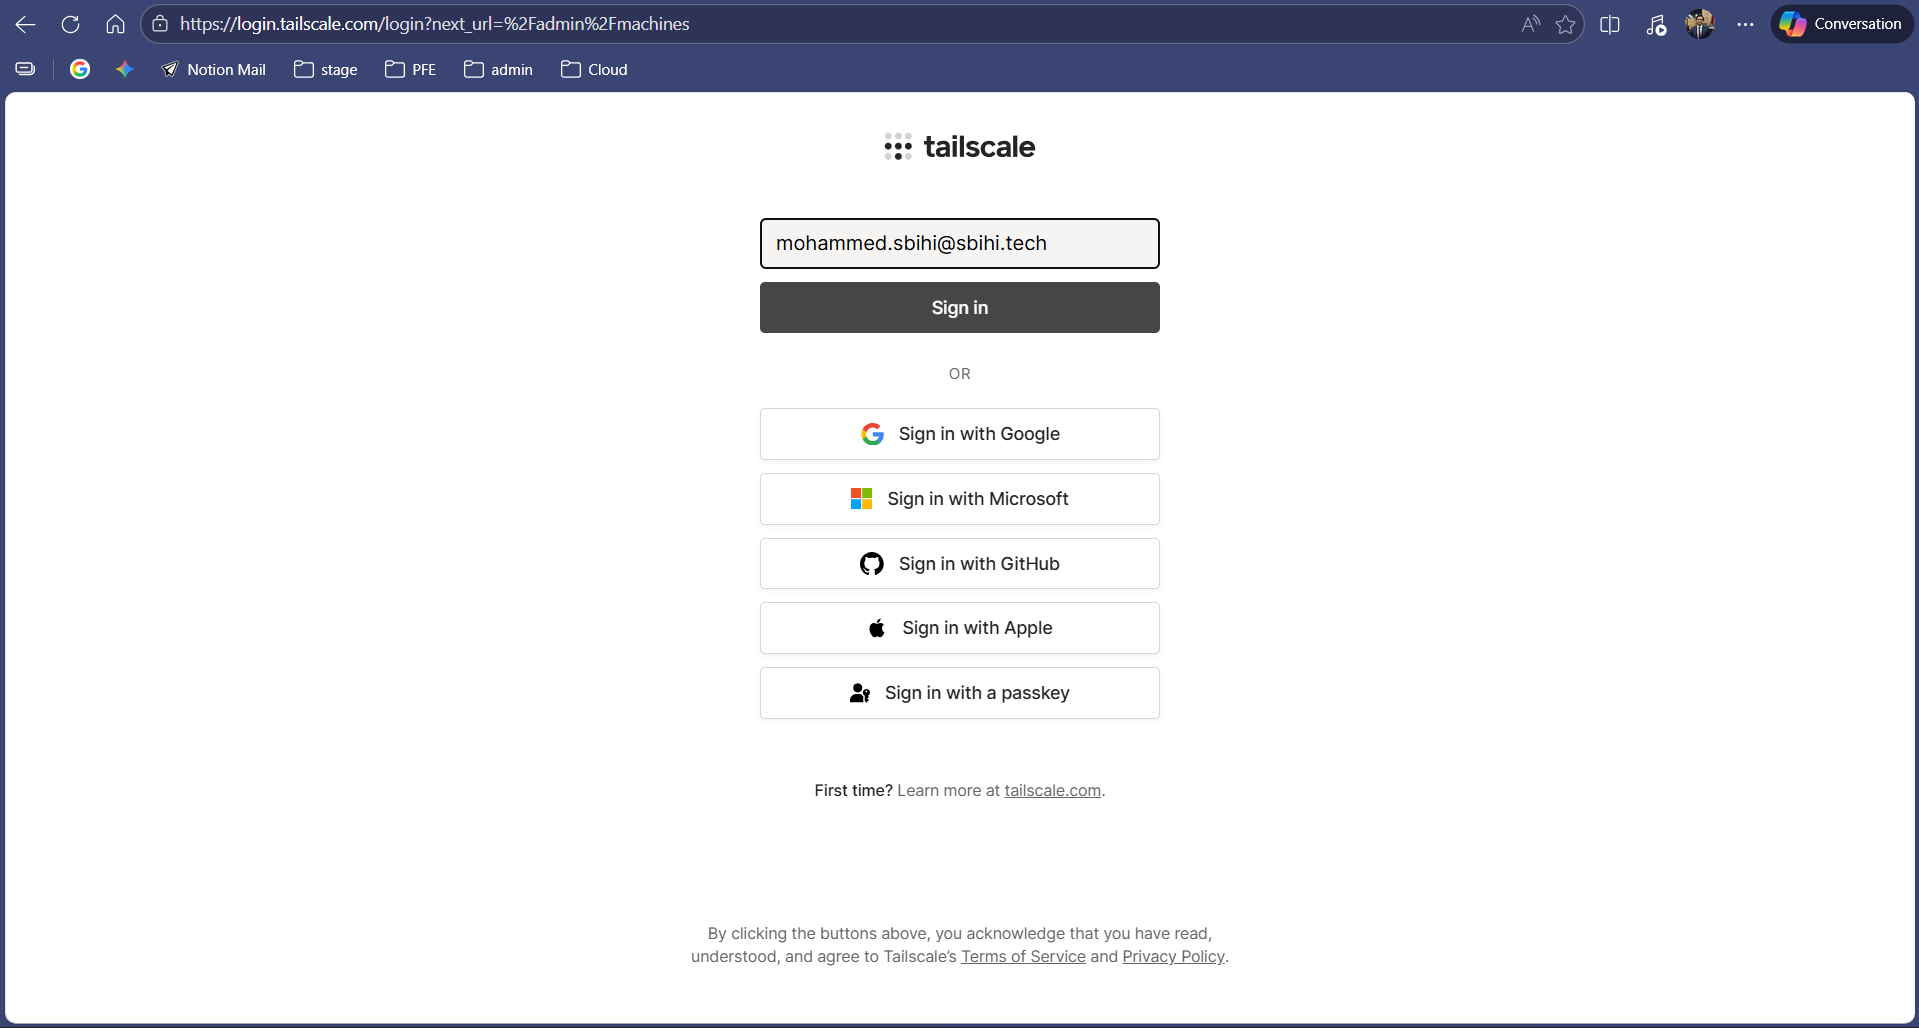
\includegraphics[width=0.82\textwidth]{images/tailscale_login/step1_enter_email.png}
	\caption{Etape 1: saisie de l'email utilisateur dans le flux de connexion Tailscale.}
	\label{fig:tailscale-step1-email}
\end{figure}
Cette ecran montre le point de depart du controle d'identite. L'utilisateur ne se connecte pas directement a la ressource cible: il initie d'abord un flux IAM, ce qui garantit que toute demande d'acces est rattachee a une identite explicite et tracable.

\begin{figure}[H]
	\centering
	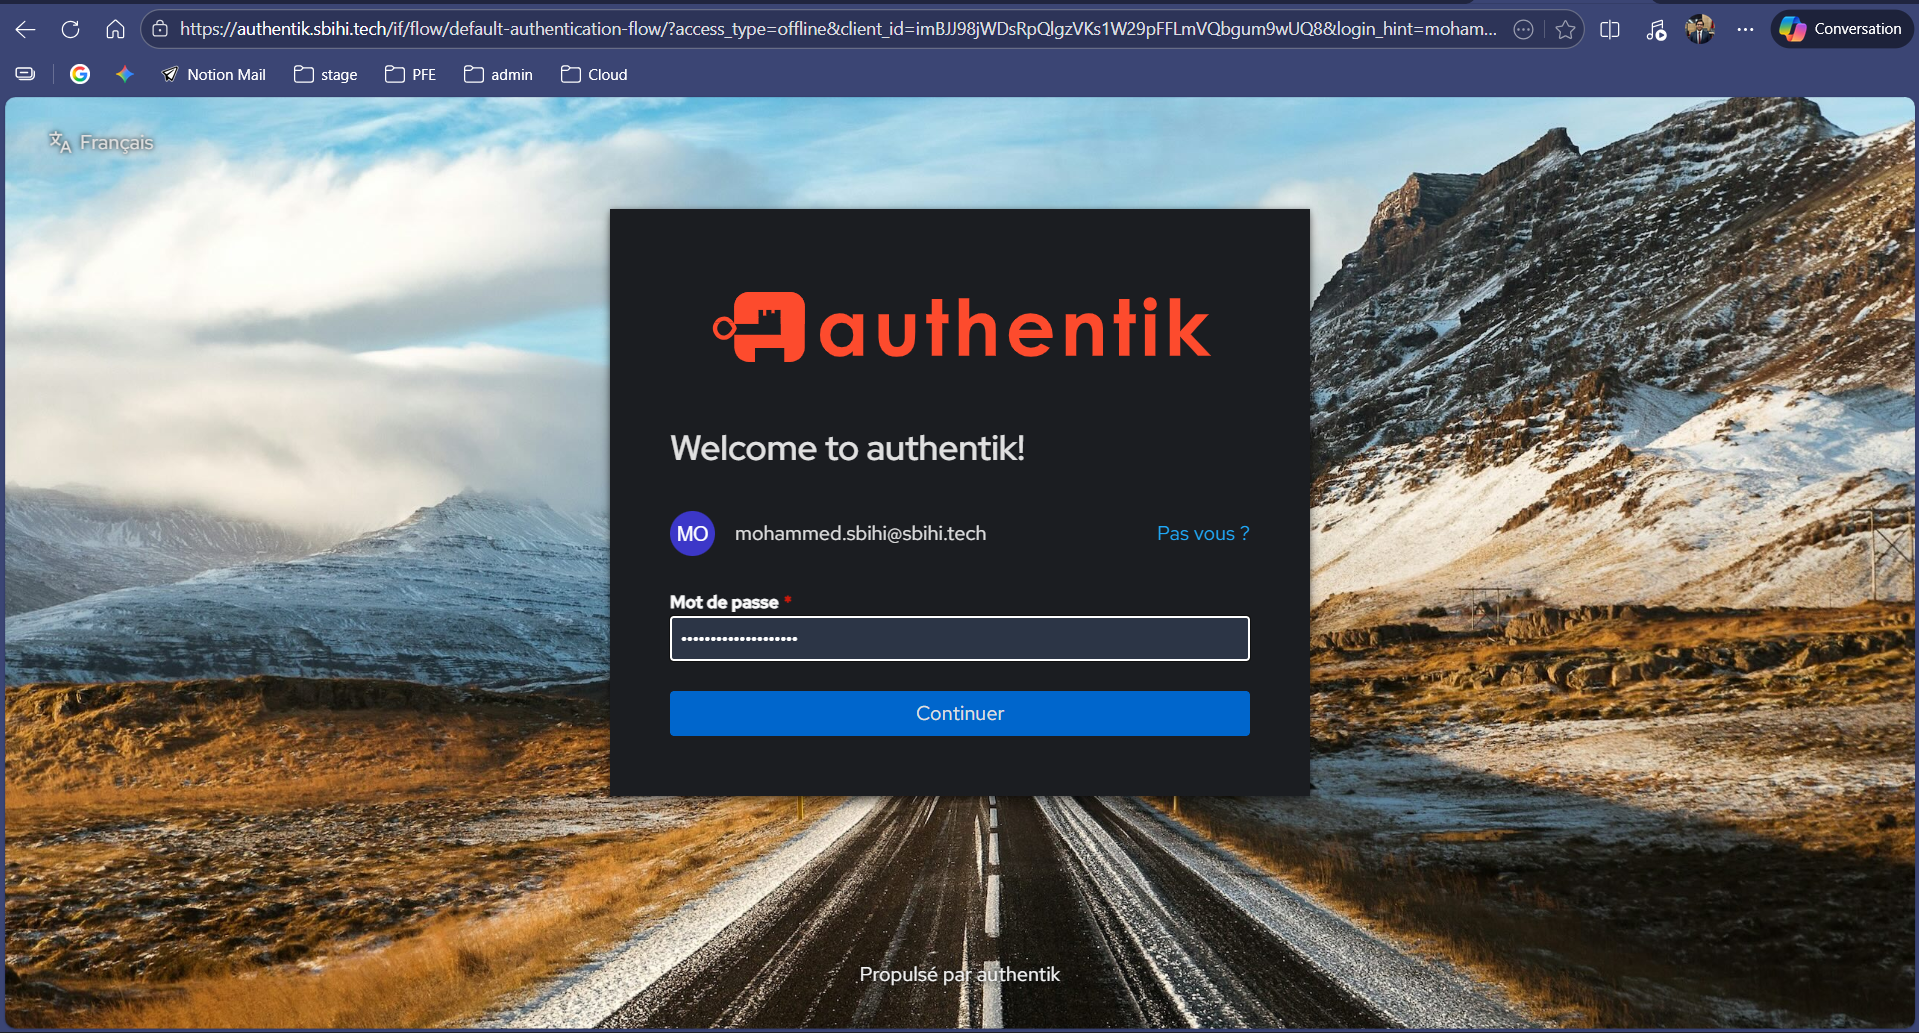
\includegraphics[width=0.82\textwidth]{images/tailscale_login/step2_rederection_to_authentik.png}
	\caption{Etape 2: redirection vers Authentik pour la verification d'identite (SSO IAM).}
	\label{fig:tailscale-step2-authentik}
\end{figure}
La redirection vers Authentik materialise la separation entre couche reseau et couche identite. Cette etape est essentielle dans Zero Trust, car la politique d'acces n'est appliquee qu'apres verification de l'identite et du contexte de connexion.

\begin{figure}[H]
	\centering
	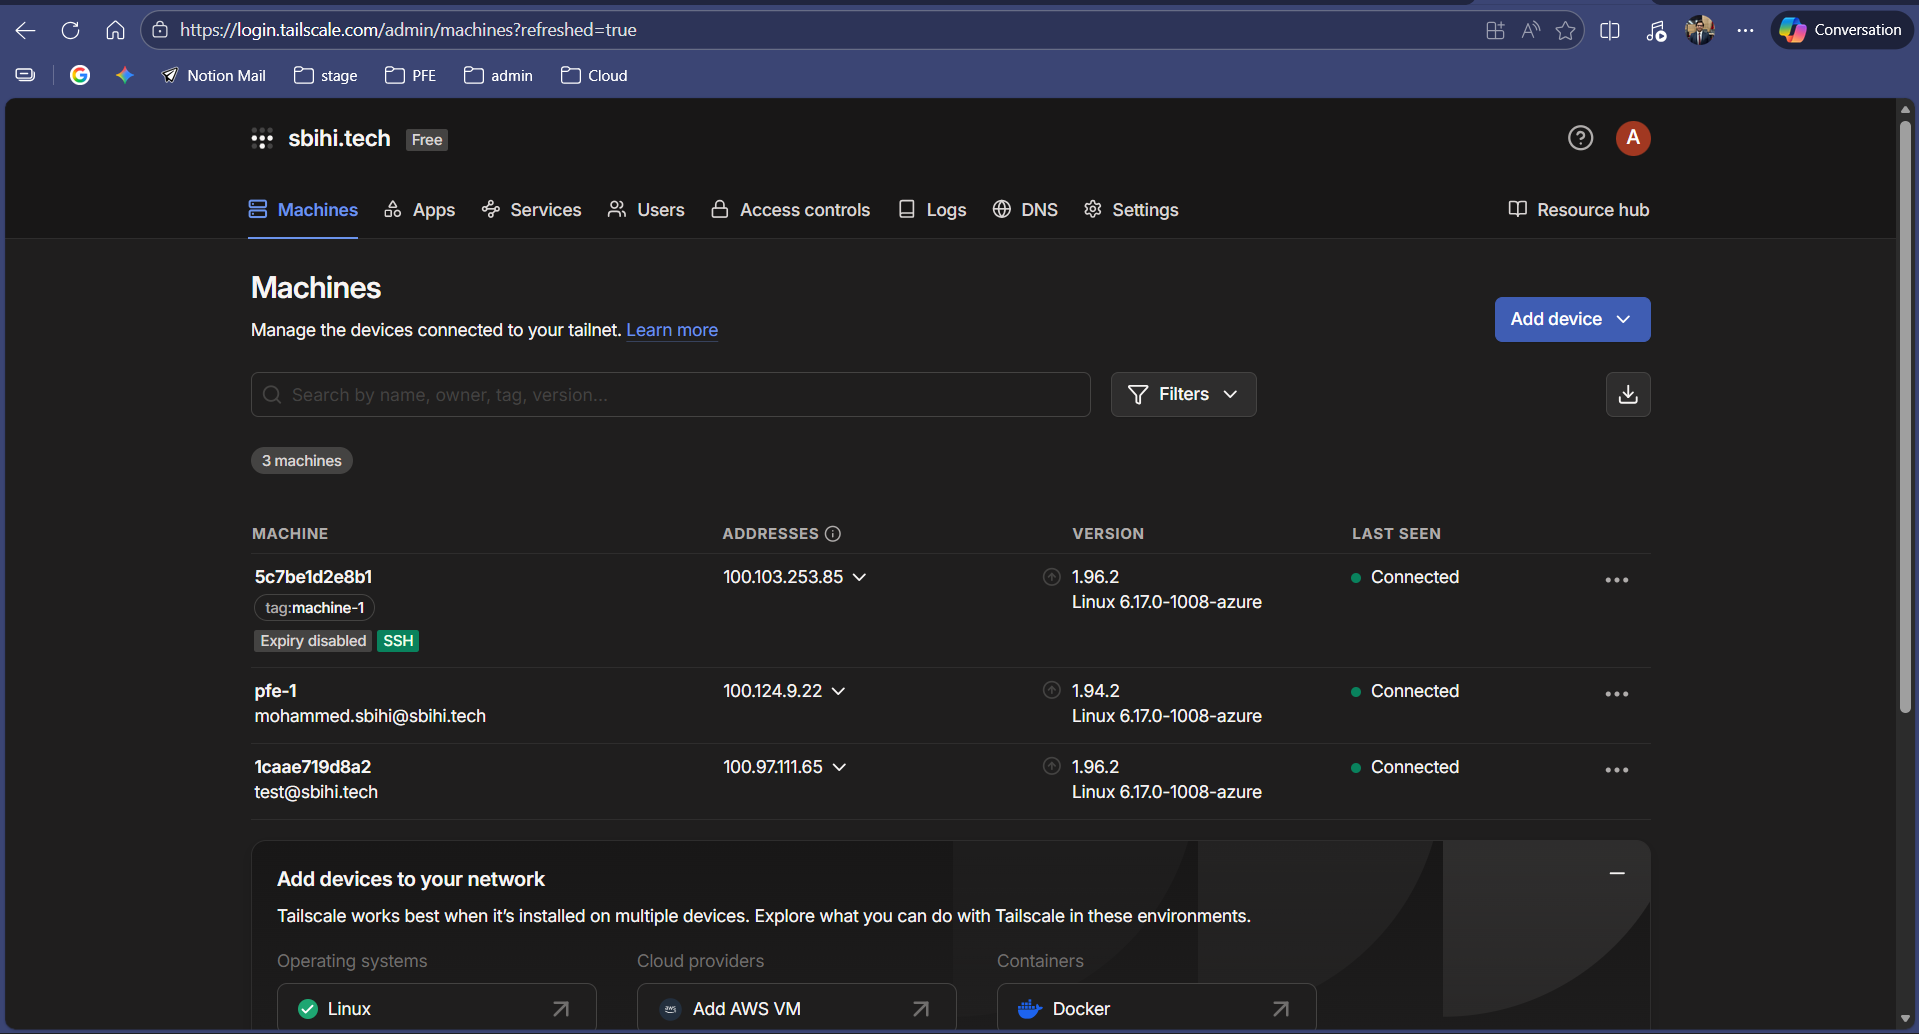
\includegraphics[width=0.82\textwidth]{images/tailscale_login/step3_back_to_tailscale.png}
	\caption{Etape 3: retour vers Tailscale apres authentification validee par Authentik.}
	\label{fig:tailscale-step3-back}
\end{figure}
Le retour vers Tailscale confirme que la federation d'authentification est correctement etablie. En pratique, cela permet de n'autoriser ensuite que les operations compatibles avec les droits du profil authentifie.

\begin{figure}[H]
	\centering
	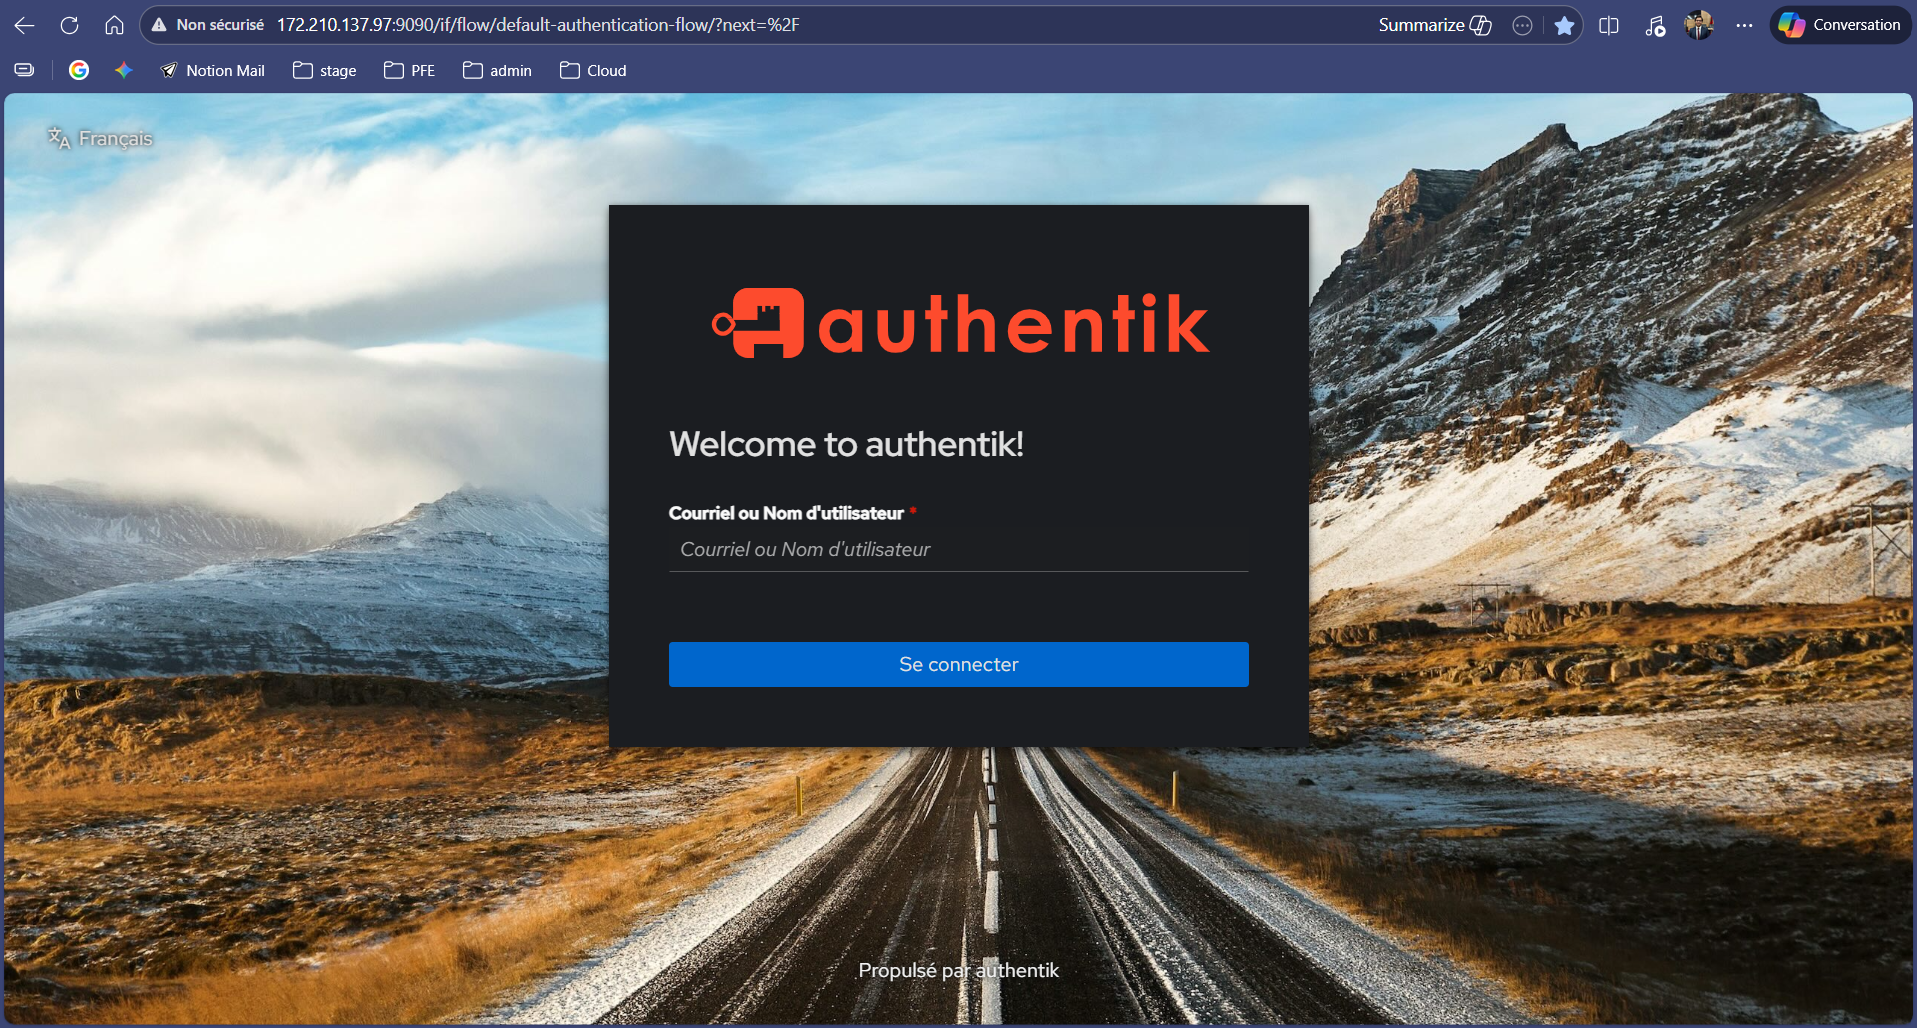
\includegraphics[width=0.9\textwidth]{images/capture de la page login.png}
	\caption{Page de connexion IAM de l'application, point d'entree du controle d'identite.}
	\label{fig:iam-login-page}
\end{figure}
Cette interface centralise l'authentification des utilisateurs de l'application de gouvernance JIT. Son role est de garantir que les actions metier (demande, approbation, revocation) sont executees par des comptes identifies et non anonymes.

\begin{figure}[H]
	\centering
	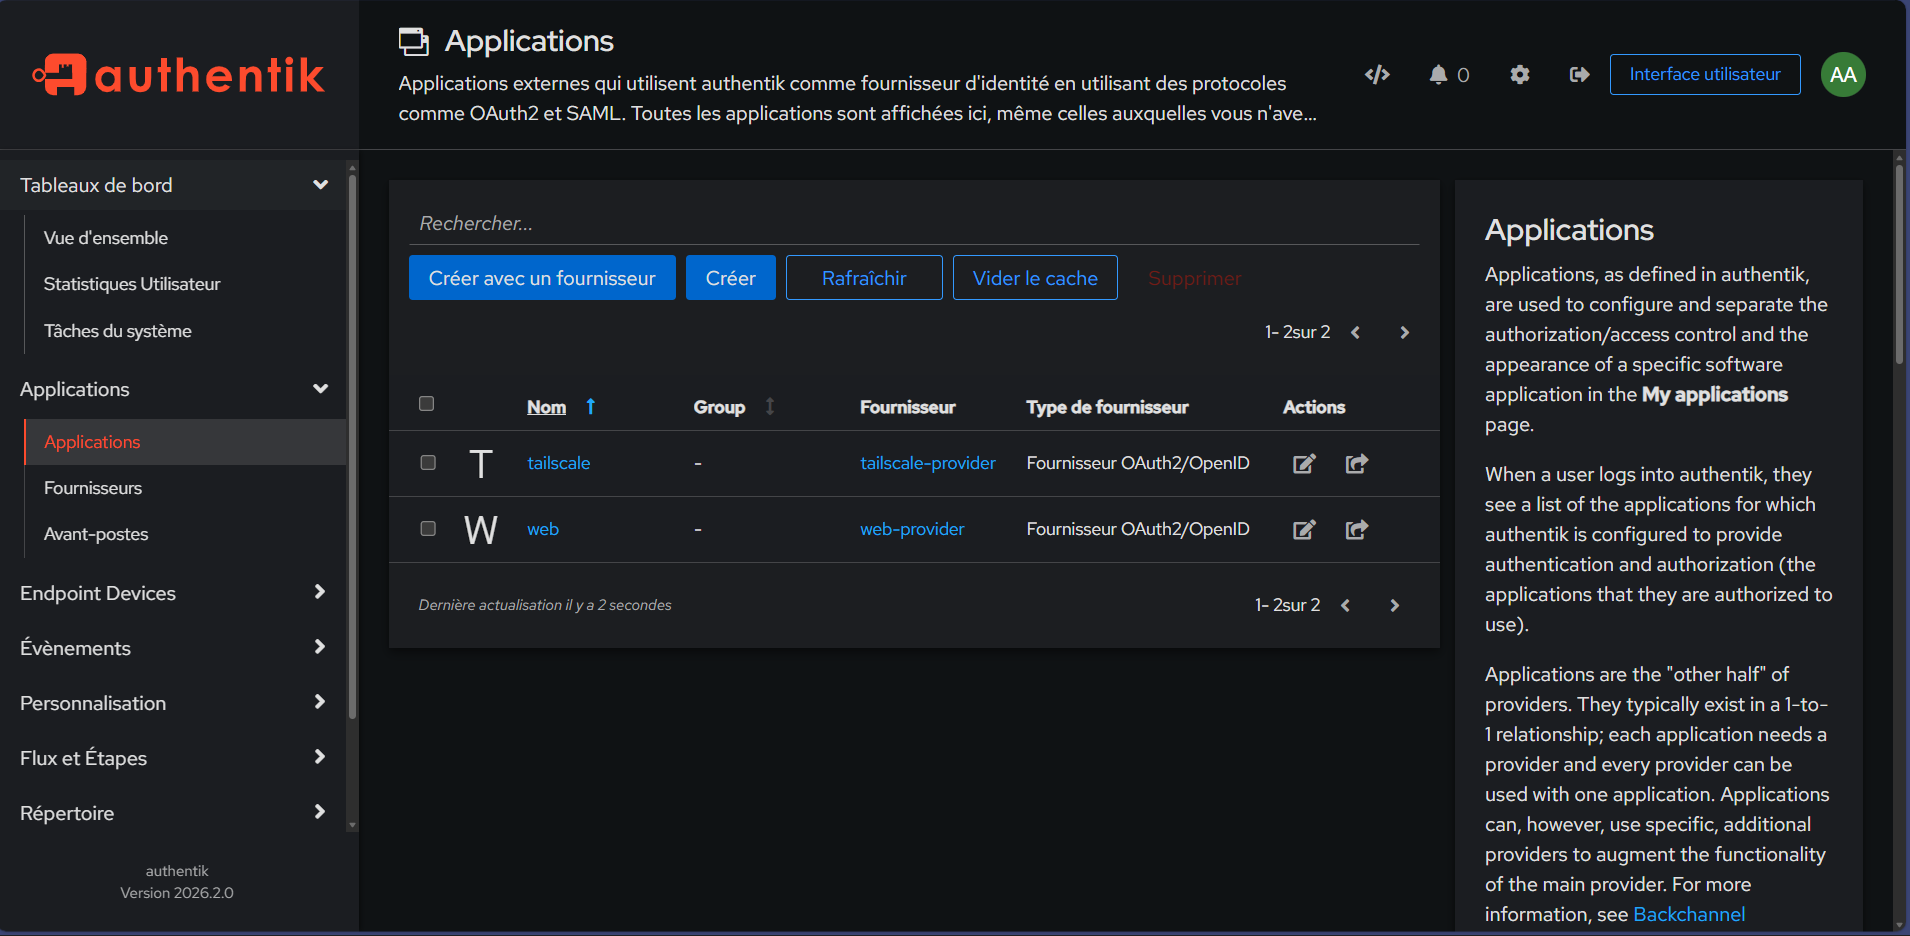
\includegraphics[width=0.9\textwidth]{images/capture de la configuration application.png}
	\caption{Configuration de l'application dans Authentik (provider, integration et parametres de federation).}
	\label{fig:iam-app-config}
\end{figure}
La configuration du provider est la piece technique qui relie le portail IAM a l'application Flask. Elle definit les URLs de redirection, les attributs transmis et les regles de confiance entre les deux systemes.

\begin{figure}[H]
	\centering
	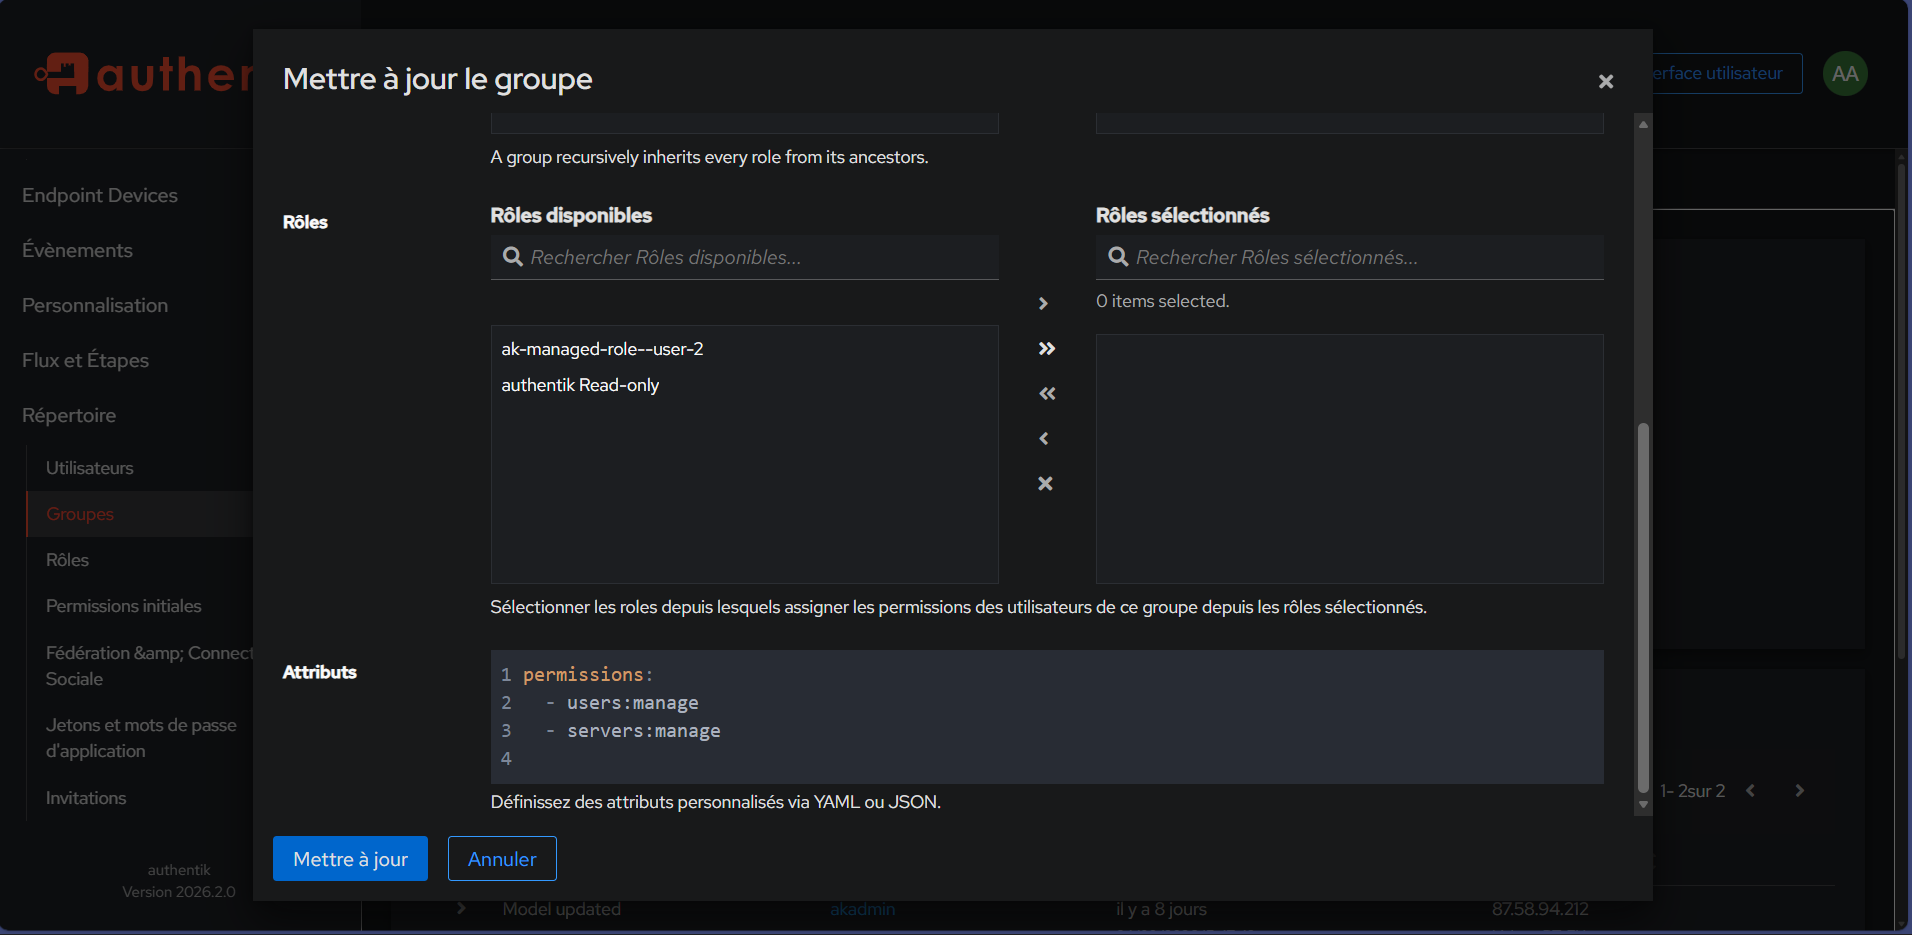
\includegraphics[width=0.9\textwidth]{images/groupes utilises pour la politique d'acces.png}
	\caption{Groupes utilises pour la politique d'acces et l'application des droits par profil.}
	\label{fig:iam-groups-policy}
\end{figure}
L'utilisation de groupes permet de decouper proprement les privileges entre utilisateurs standards et administrateurs. Ce modele facilite l'audit, car chaque droit peut etre justifie par l'appartenance a un groupe metier defini.

\section{Tailscale ACL (controle reseau)}
Tailscale est utilise comme couche de controle reseau Zero Trust avec ACL explicites.

Les points clefs de configuration sont:
\begin{itemize}
	\item etiquetage des machines cibles (tags d'environnement et de criticite);
	\item regles ACL fondees sur l'identite/groupe et la machine cible;
	\item ouverture d'acces strictement conditionnee a l'approbation JIT.
\end{itemize}

L'effet recherche est binaire et verifiable:
\begin{itemize}
	\item avant approbation JIT: acces refuse;
	\item apres approbation JIT: acces autorise pendant la fenetre TTL;
	\item apres expiration TTL: acces de nouveau refuse.
\end{itemize}

\begin{figure}[H]
	\centering
	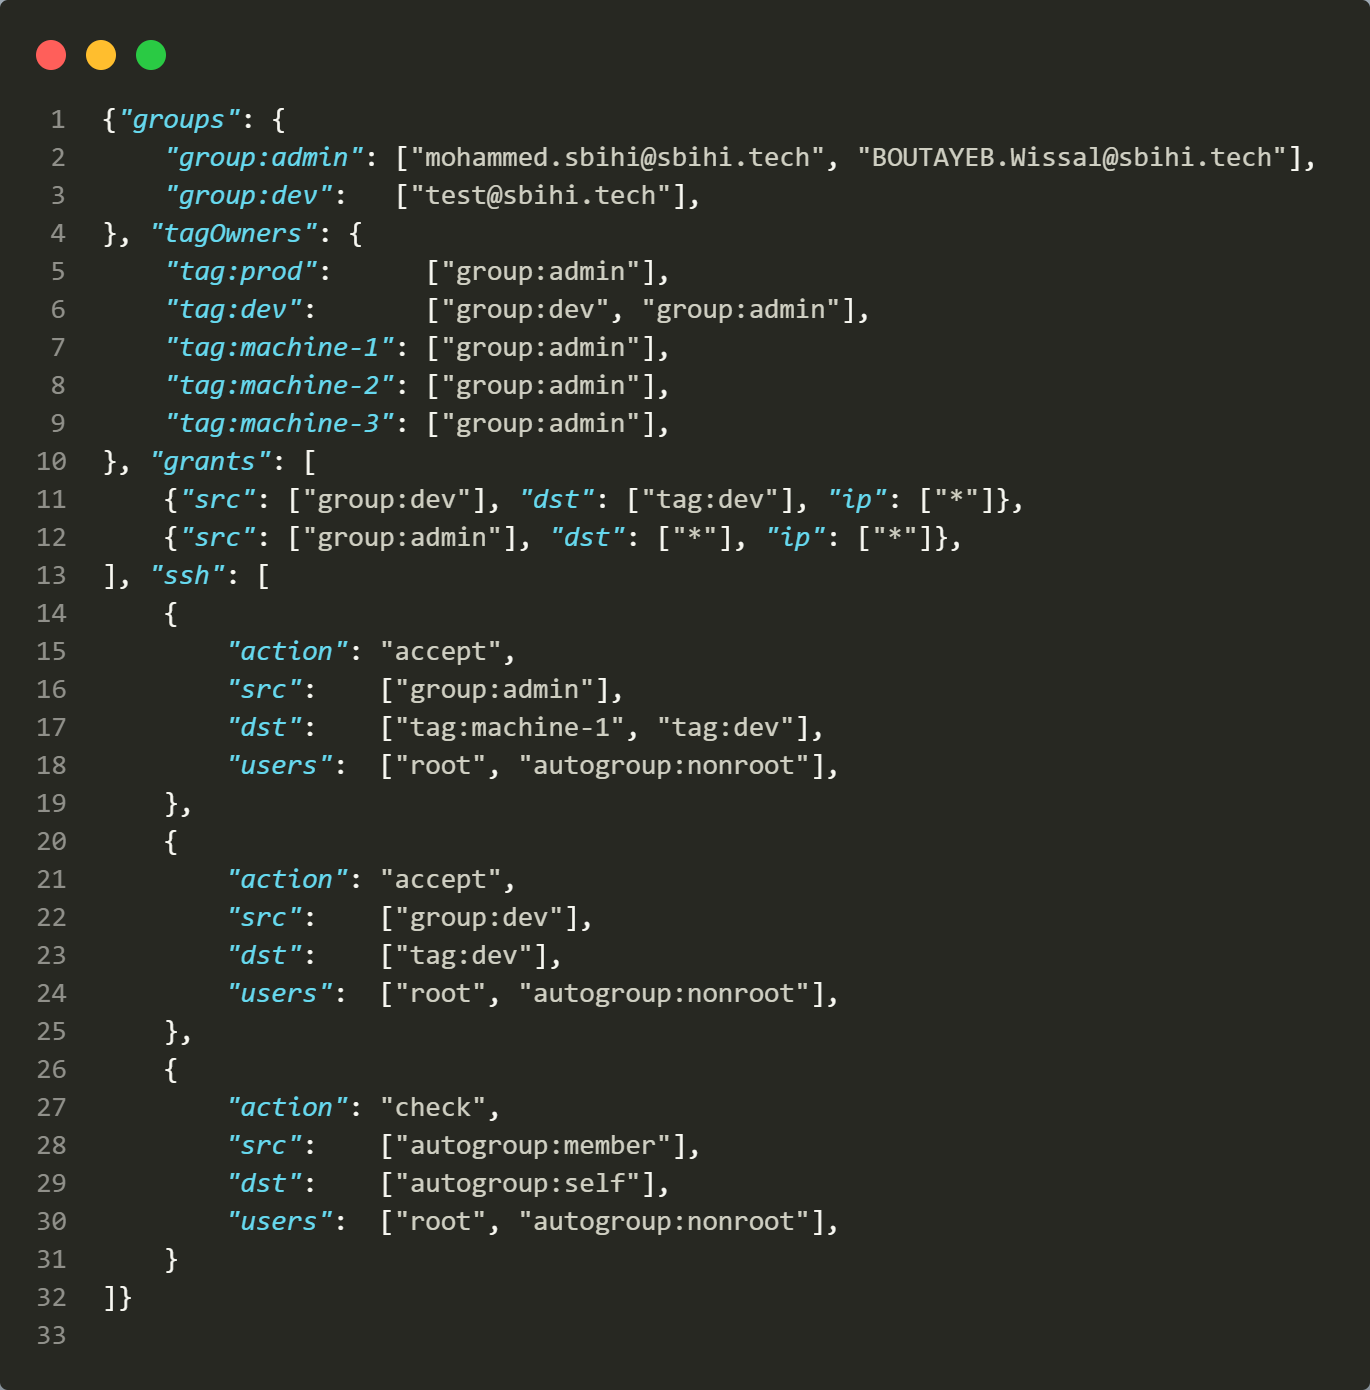
\includegraphics[width=0.95\textwidth]{images/acl-before-acces-granted.png}
	\caption{Etat ACL avant approbation: politique restrictive, sans autorisation explicite pour l'utilisateur cible.}
	\label{fig:acl-before-grant}
\end{figure}
Cette capture illustre le principe de base du modele Zero Trust: l'absence d'autorisation explicite equivaut a un refus d'acces. L'utilisateur ne peut donc pas atteindre la cible tant que la gouvernance JIT n'a pas valide la demande.

\begin{figure}[H]
	\centering
	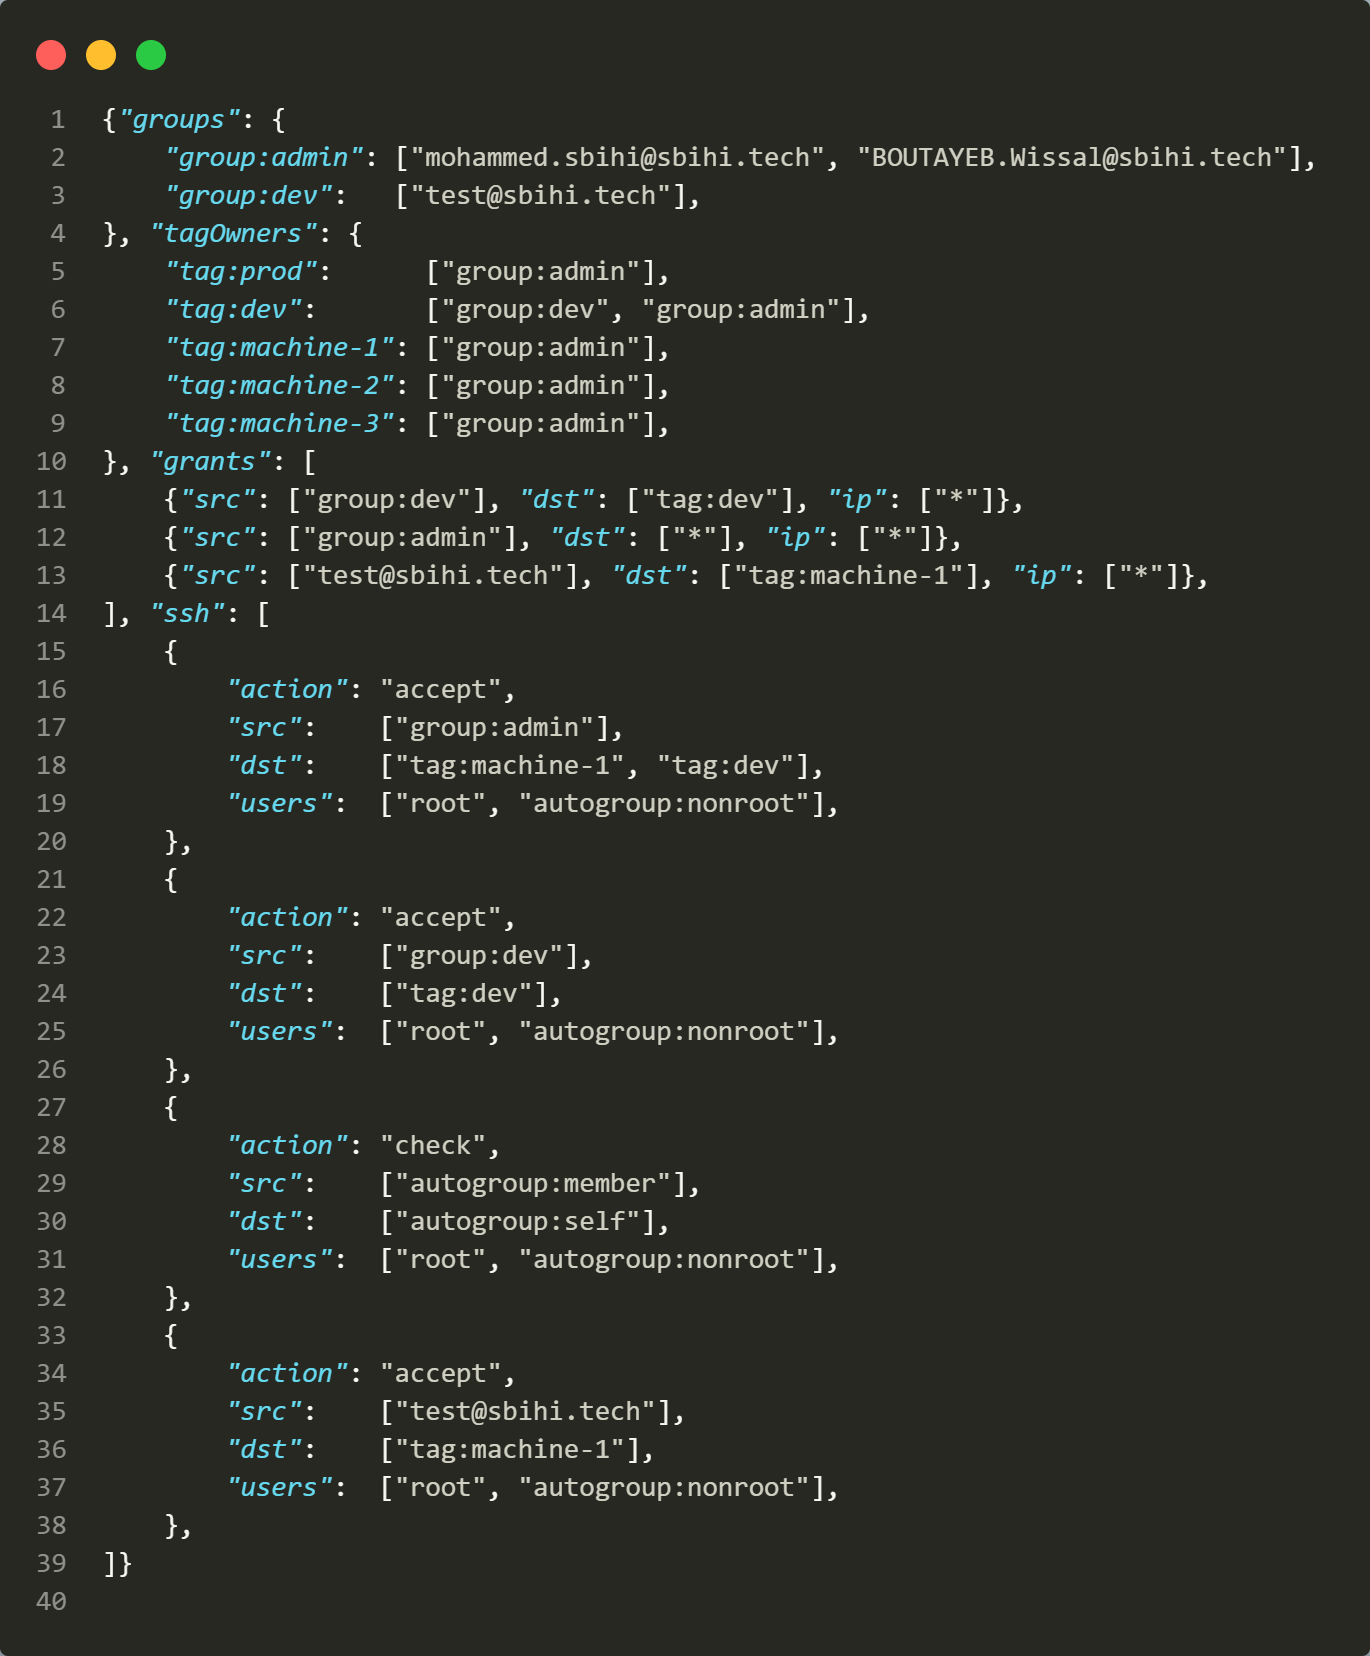
\includegraphics[width=0.95\textwidth]{images/acl-after-acces-granted.png}
	\caption{Etat ACL apres approbation: regle d'acces temporaire ajoutee pour permettre la connexion.}
	\label{fig:acl-after-grant}
\end{figure}
Apres approbation, l'ajout de la regle ACL prouve la transition controlee de l'etat refuse vers l'etat autorise. Le changement n'est pas permanent: il est lie a une demande, une justification et une fenetre temporelle limitee.

\begin{figure}[H]
	\centering
	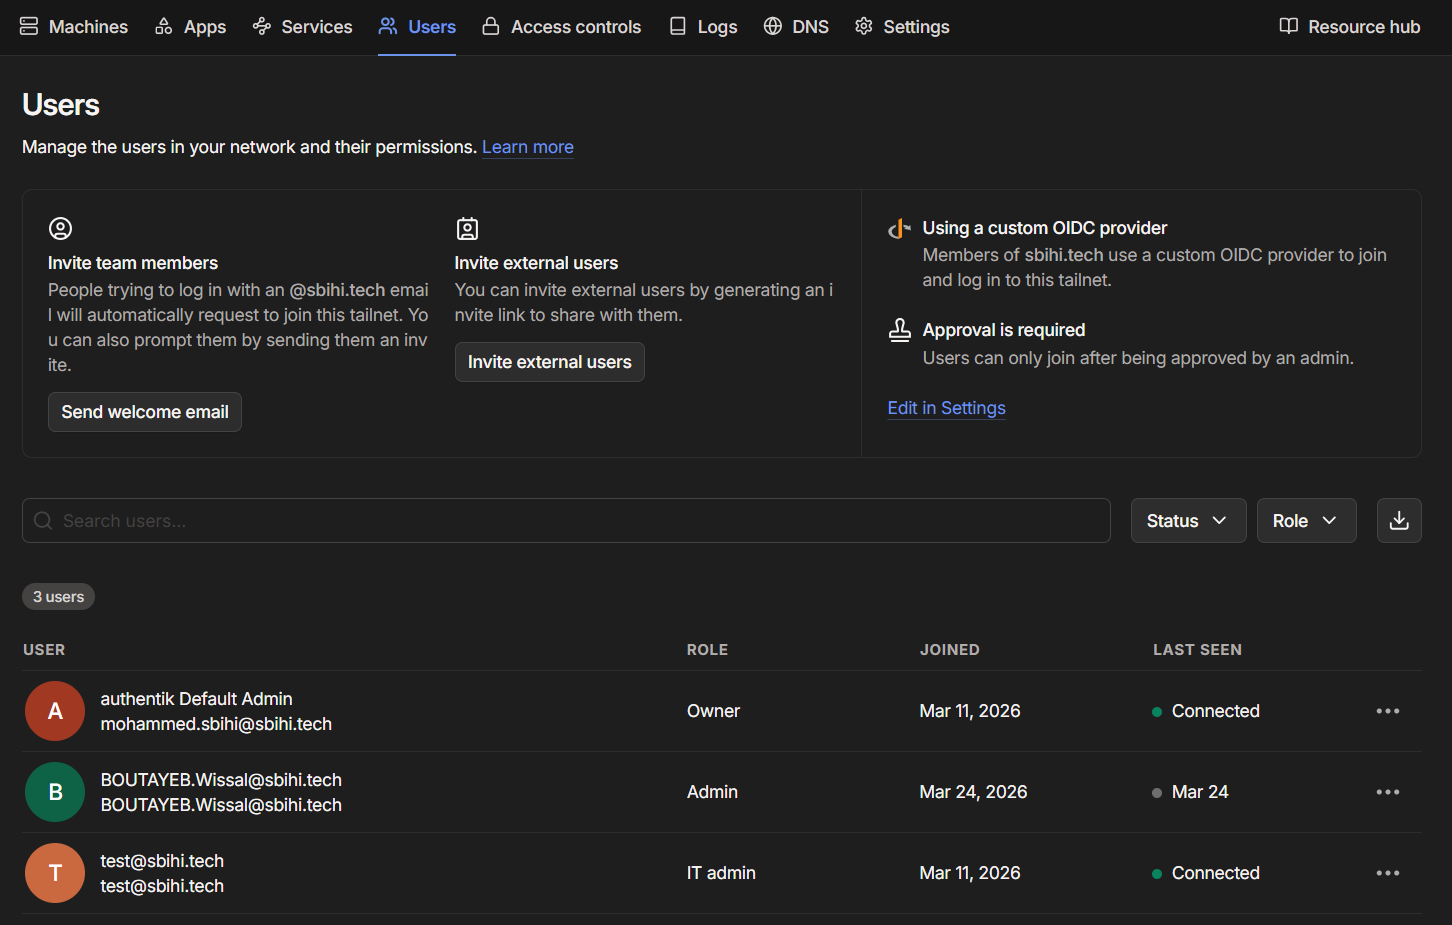
\includegraphics[width=0.9\textwidth]{images/list_of_users_in_tailscale.png}
	\caption{Vue des utilisateurs Tailscale, utilisee pour verifier les identites effectives dans le tailnet.}
	\label{fig:tailscale-users-list}
\end{figure}
La liste des utilisateurs dans le tailnet sert de point de controle supplementaire pour verifier la coherence entre identites IAM et identites reseau. Cette coherence est indispensable pour appliquer des ACL precises et non ambiguës.

\section{Application Flask et base PostgreSQL}
L'application web implemente le cycle de vie des demandes d'acces privilegie.

Les statuts metier principaux sont:
\begin{itemize}
	\item \texttt{pending}: demande en attente d'approbation;
	\item \texttt{approved}: demande acceptee avec expiration;
	\item \texttt{denied}: demande refusee;
	\item \texttt{expired}: acces arrive a echeance.
\end{itemize}

Les regles metier importantes sont:
\begin{itemize}
	\item blocage des doublons \texttt{pending} pour une meme cible/utilisateur;
	\item affichage de l'etat courant et du temps restant pour les acces actifs;
	\item separation des interfaces \textit{user side} et \textit{admin side}.
\end{itemize}

Les ecrans suivants montrent la separation des responsabilites entre utilisateur et administrateur.

\begin{figure}[H]
	\centering
	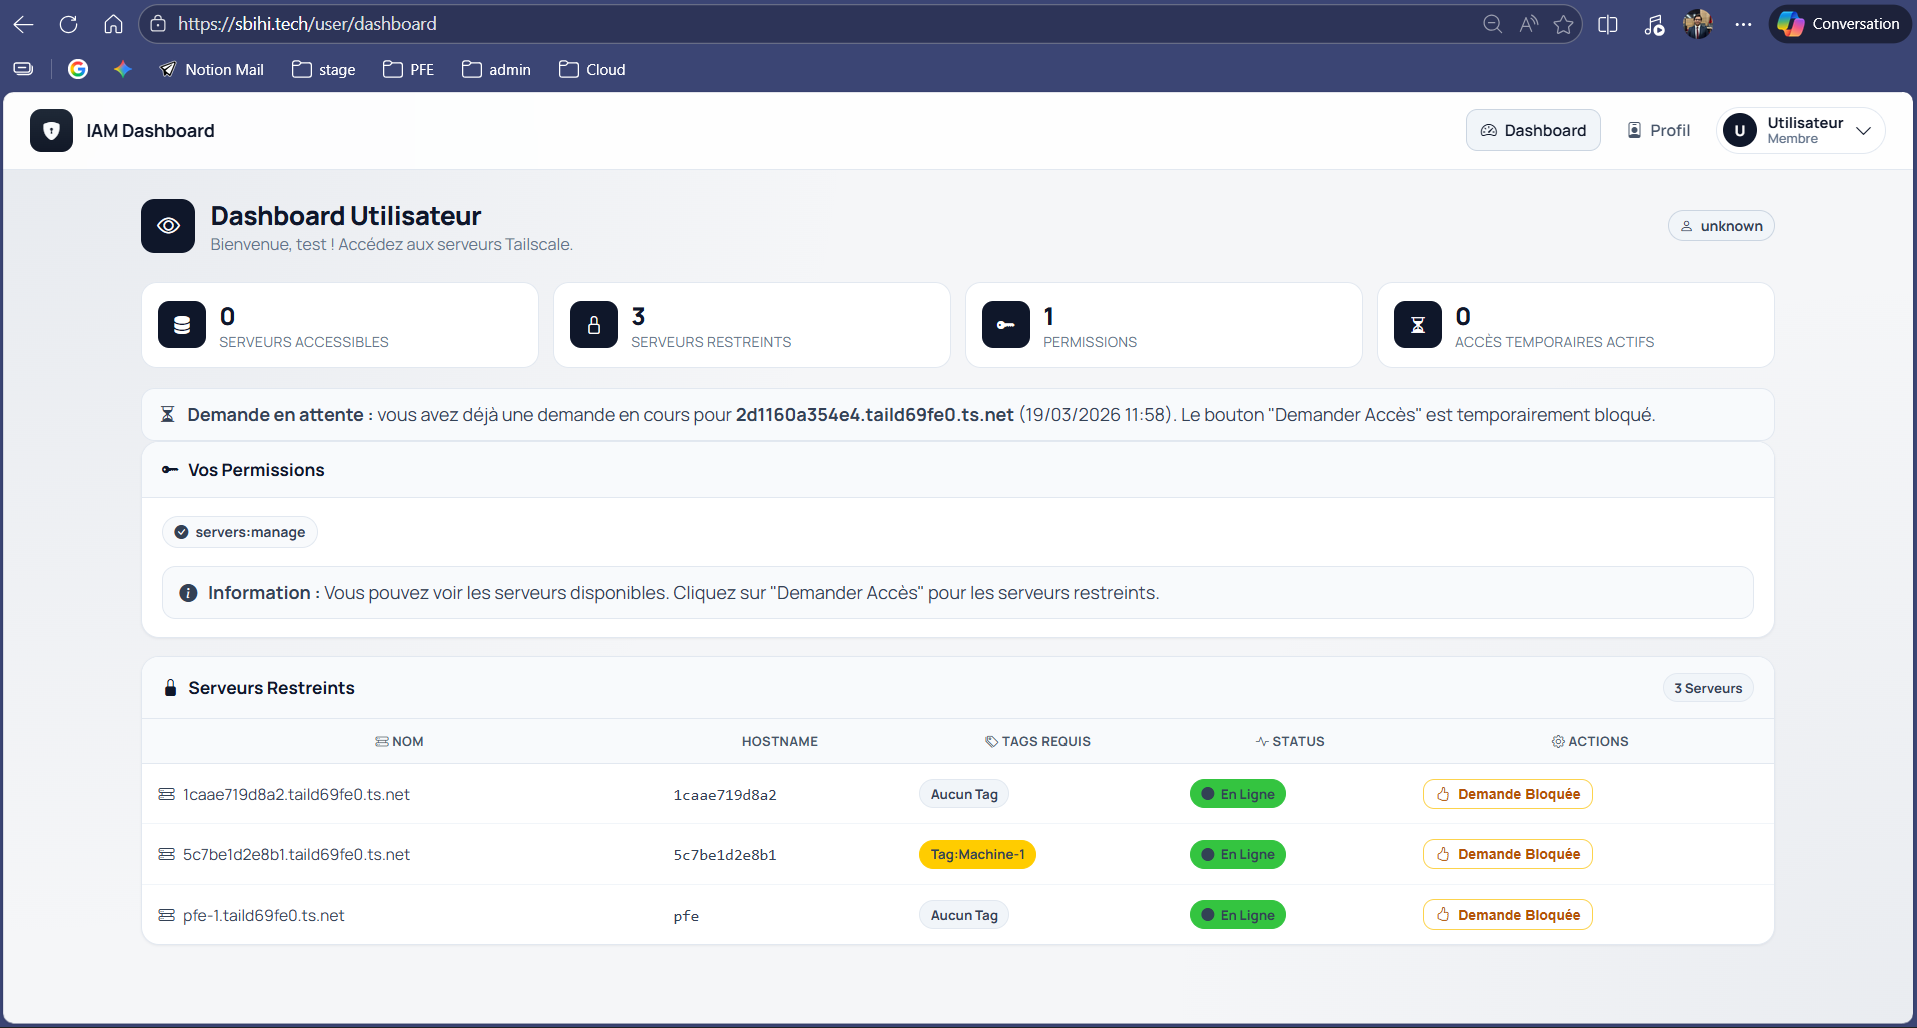
\includegraphics[width=0.95\textwidth]{images/iam_test_dashbord.png}
	\caption{Dashboard utilisateur (user side): consultation de l'etat des acces et lancement d'une demande JIT.}
	\label{fig:user-dashboard}
\end{figure}
Le tableau de bord utilisateur expose uniquement les operations necessaires au role demandeur. Cette limitation de surface fonctionnelle reduit les risques d'erreur et respecte le principe de moindre privilege au niveau applicatif.

\begin{figure}[H]
	\centering
	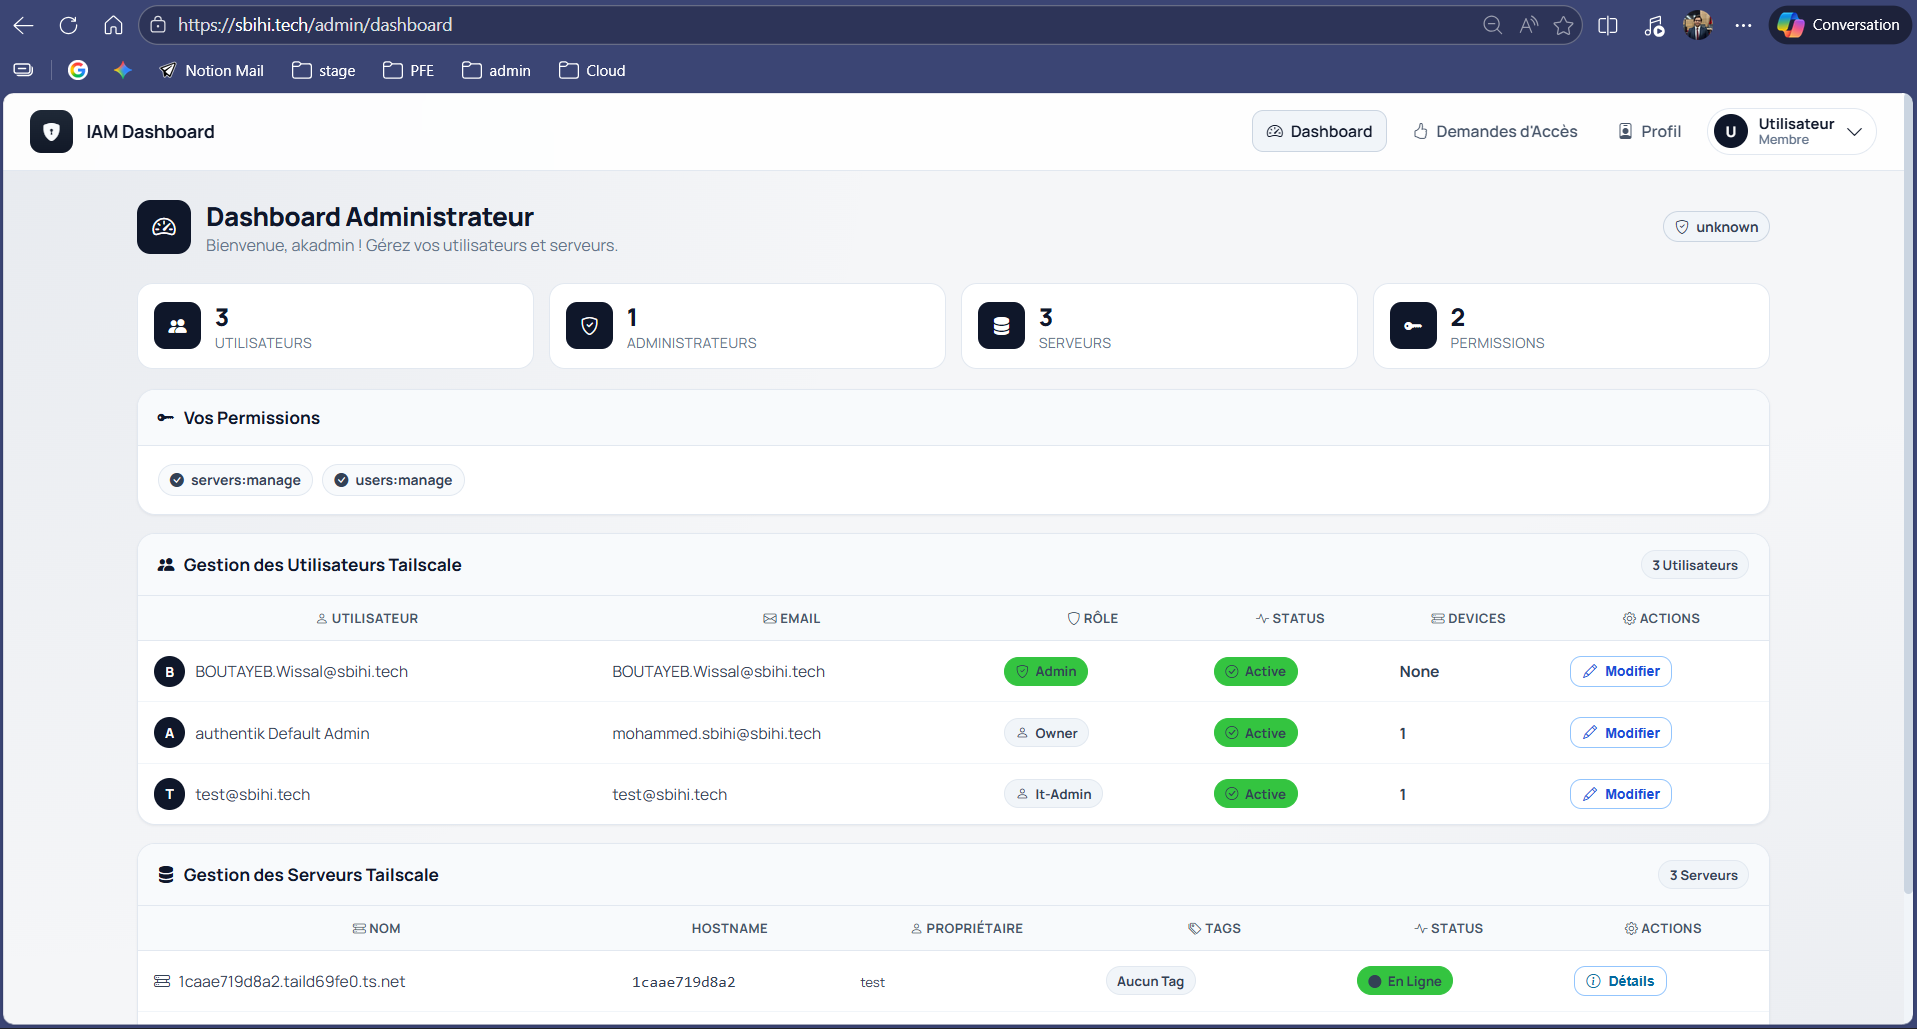
\includegraphics[width=0.95\textwidth]{images/iam_admin_dashbord.png}
	\caption{Dashboard administrateur (admin side): supervision globale des demandes et des actions de gouvernance.}
	\label{fig:admin-dashboard}
\end{figure}
Le tableau de bord administrateur centralise les decisions de gouvernance: validation, refus et suivi des demandes. Il constitue le point de pilotage des privileges temporaires accordes sur l'infrastructure.

\begin{figure}[H]
	\centering
	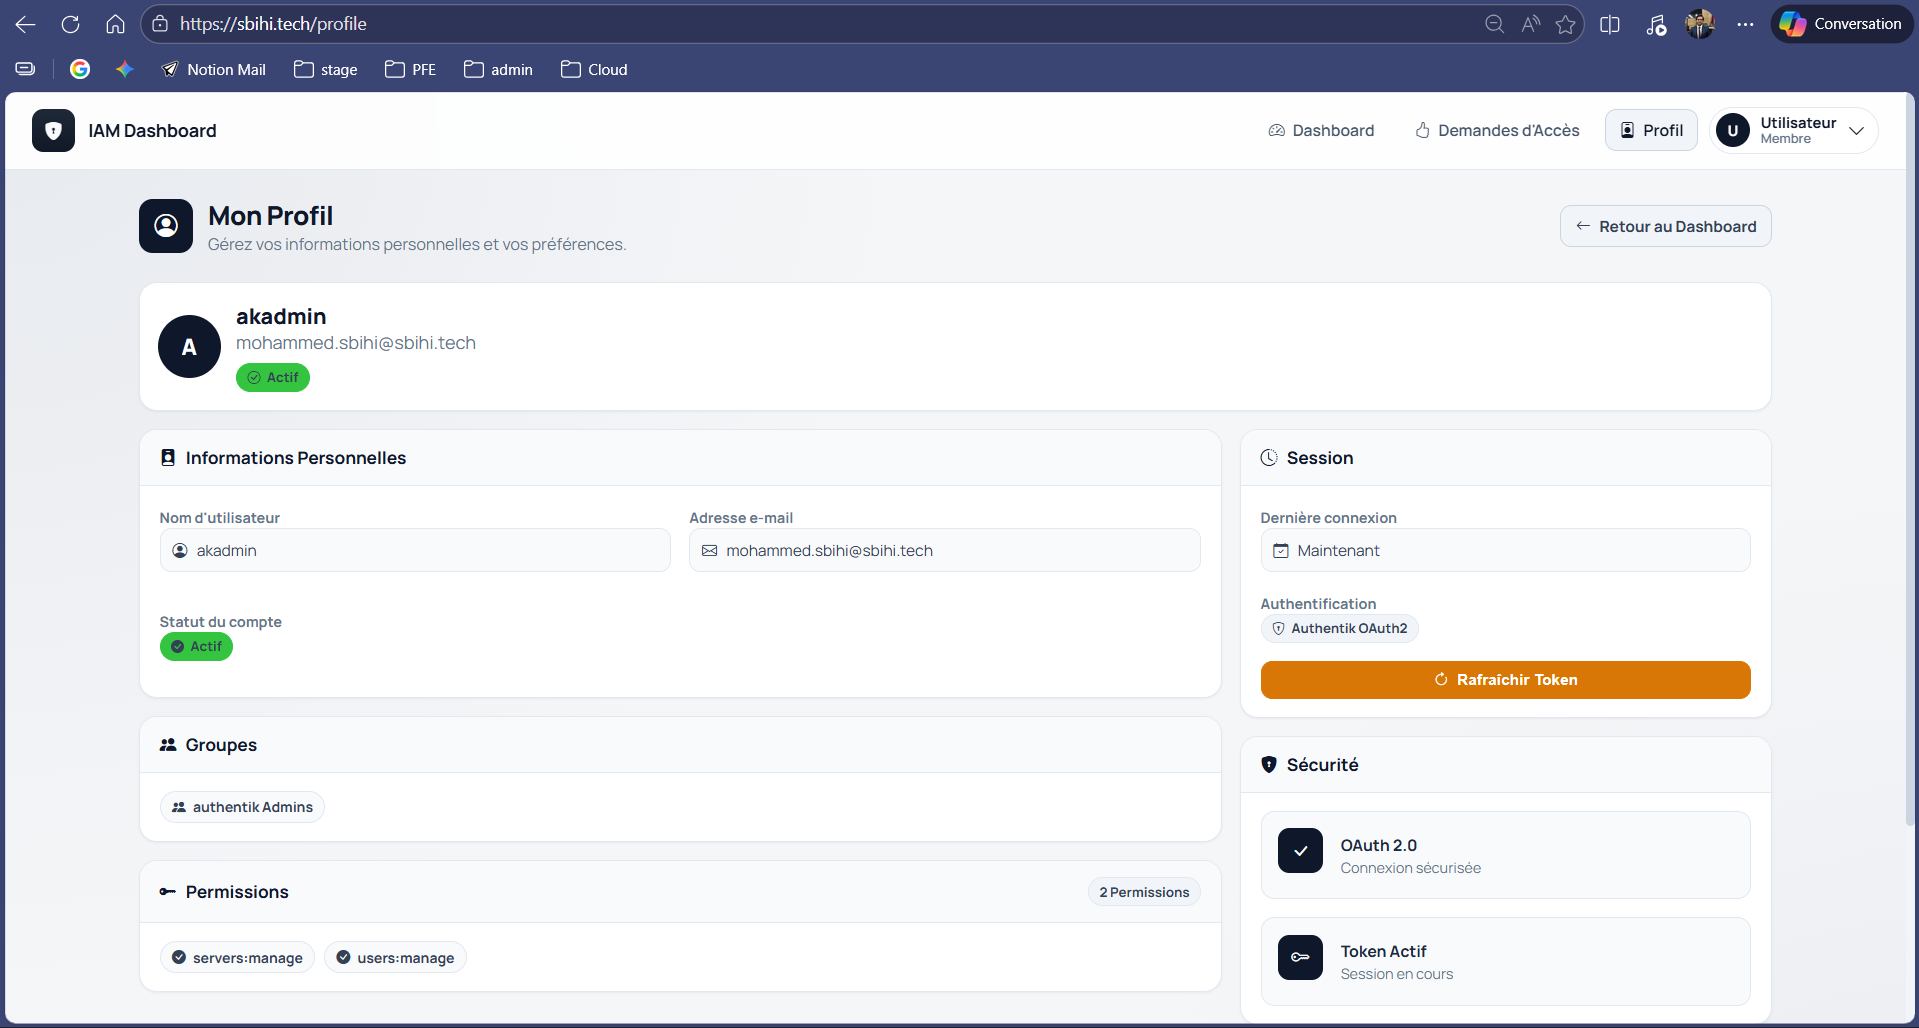
\includegraphics[width=0.95\textwidth]{images/iam_admin_dashbord_profile.png}
	\caption{Vue profil admin: verification des attributs d'identite et des permissions associees au role administrateur.}
	\label{fig:admin-profile}
\end{figure}
La vue profil admin permet de verifier les attributs d'identite utiles a l'audit: roles, groupe et informations de compte. Elle est utile pour confirmer que l'approbation est realisee par un acteur habilite.

\begin{figure}[H]
	\centering
	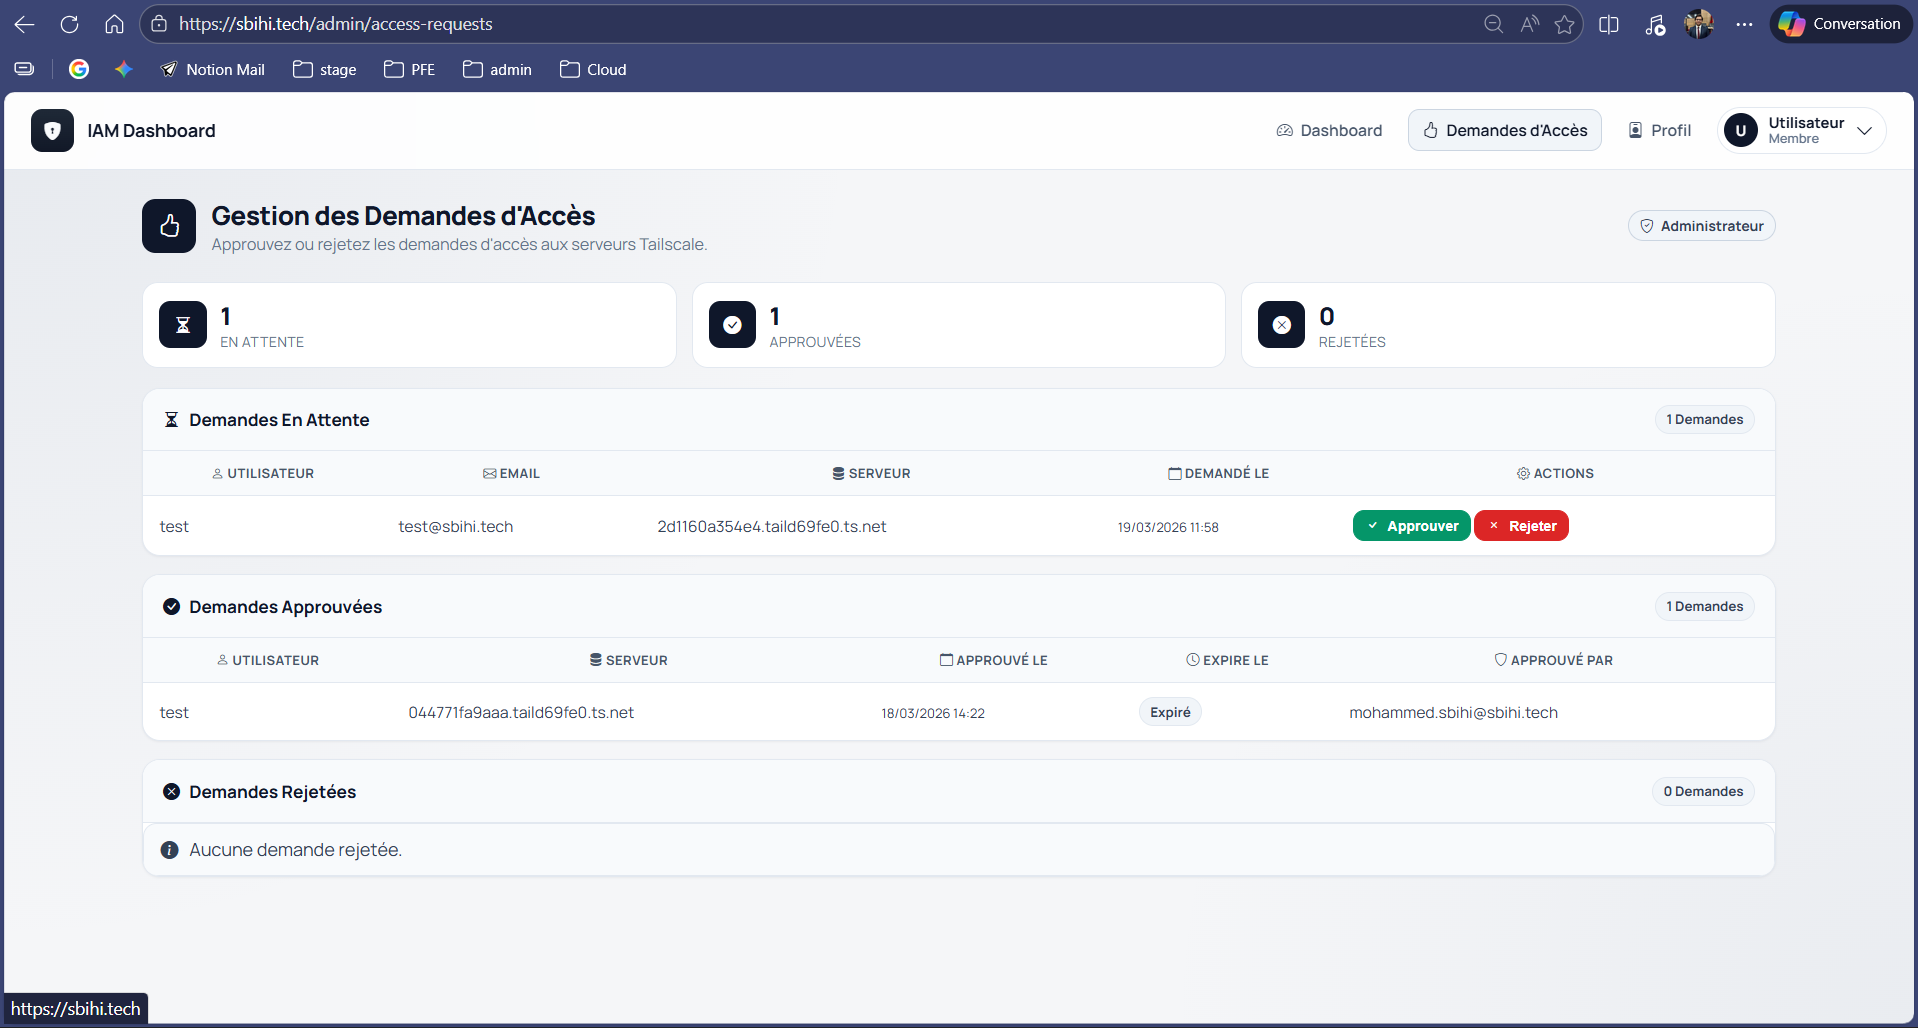
\includegraphics[width=0.95\textwidth]{images/iam_admin_dashbord_acces_request_admin.png}
	\caption{Interface de traitement des demandes d'acces cote admin (liste des requetes et statut).}
	\label{fig:admin-requests-list}
\end{figure}
La file des demandes fournit une vue operationnelle sur les etats \texttt{pending}, \texttt{approved} et \texttt{denied}. Cette visibilite facilite la priorisation des actions et le respect des delais de traitement.

\begin{figure}[H]
	\centering
	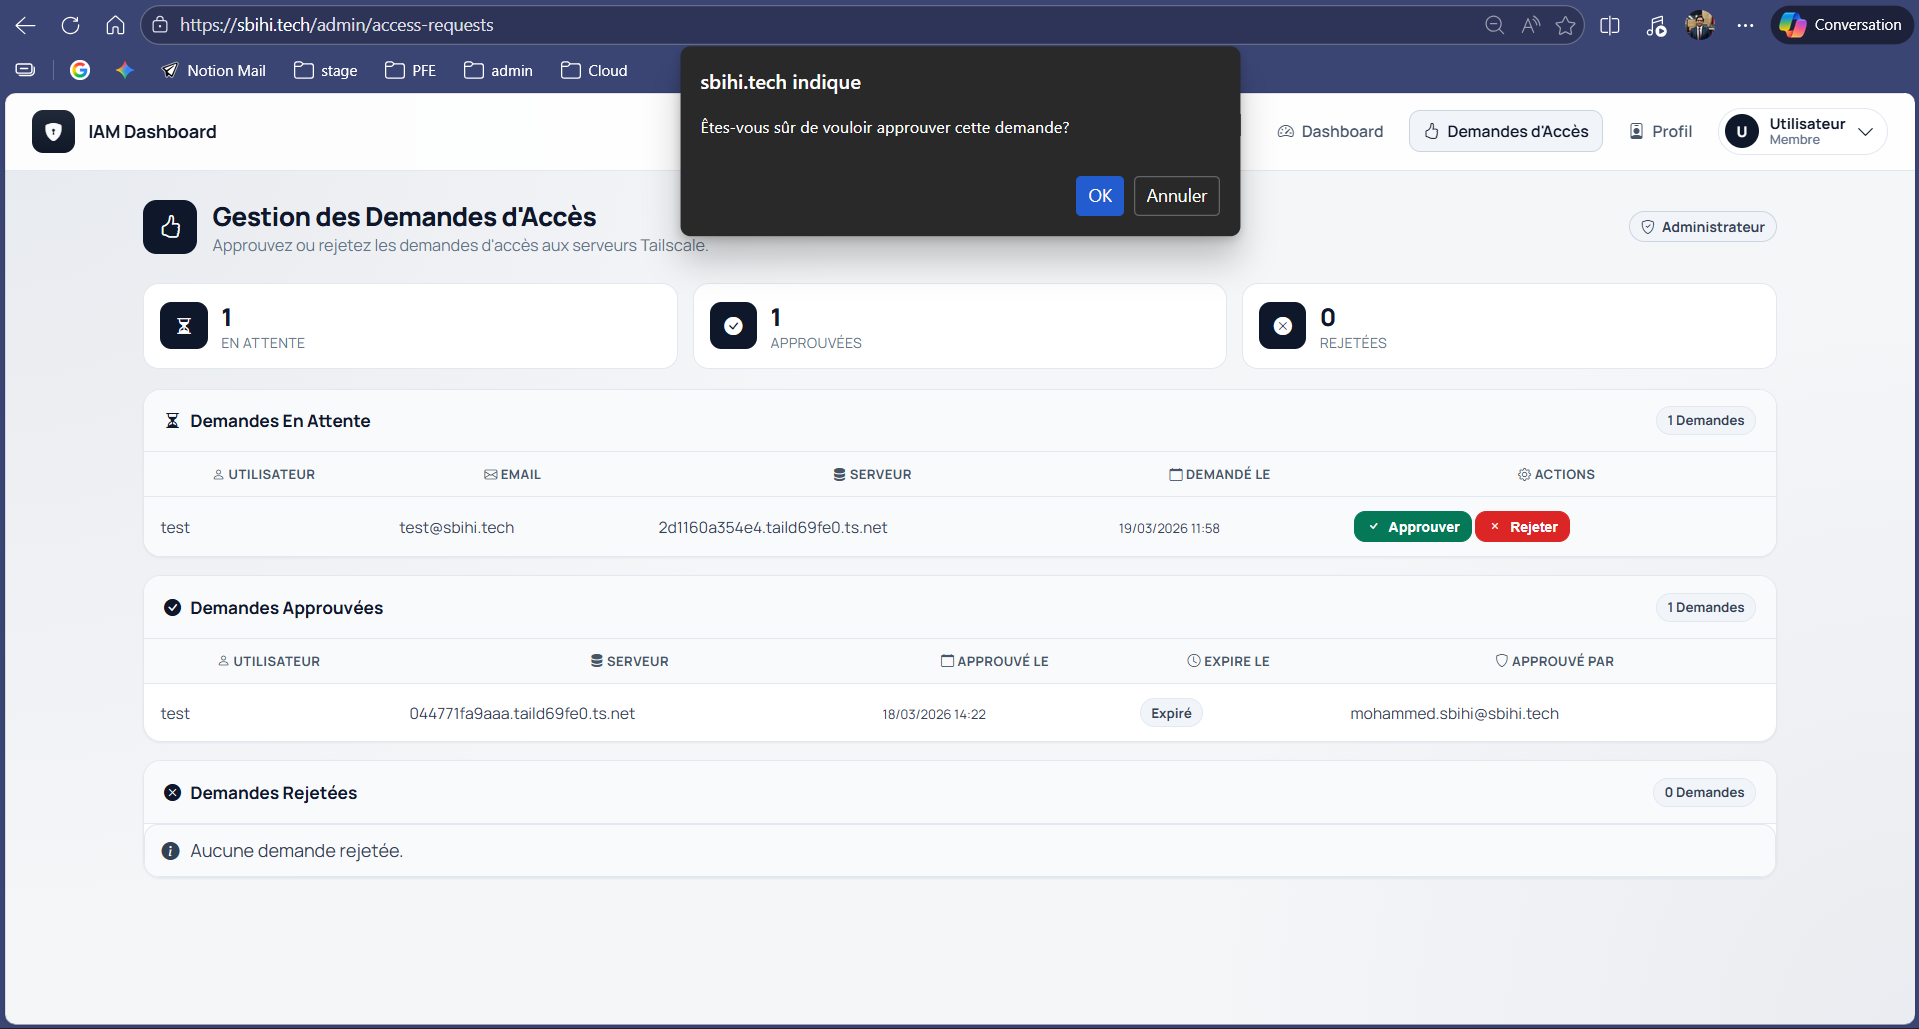
\includegraphics[width=0.95\textwidth]{images/approuve_request_by_admin.png}
	\caption{Action d'approbation d'une demande par l'administrateur, declenchant l'activation ACL temporaire.}
	\label{fig:admin-approve-action}
\end{figure}
Cette preuve met en evidence le point de bascule du workflow JIT. L'approbation ne donne pas un droit global: elle genere un droit cible, borne dans le temps, et directement traçable.

\begin{figure}[H]
	\centering
	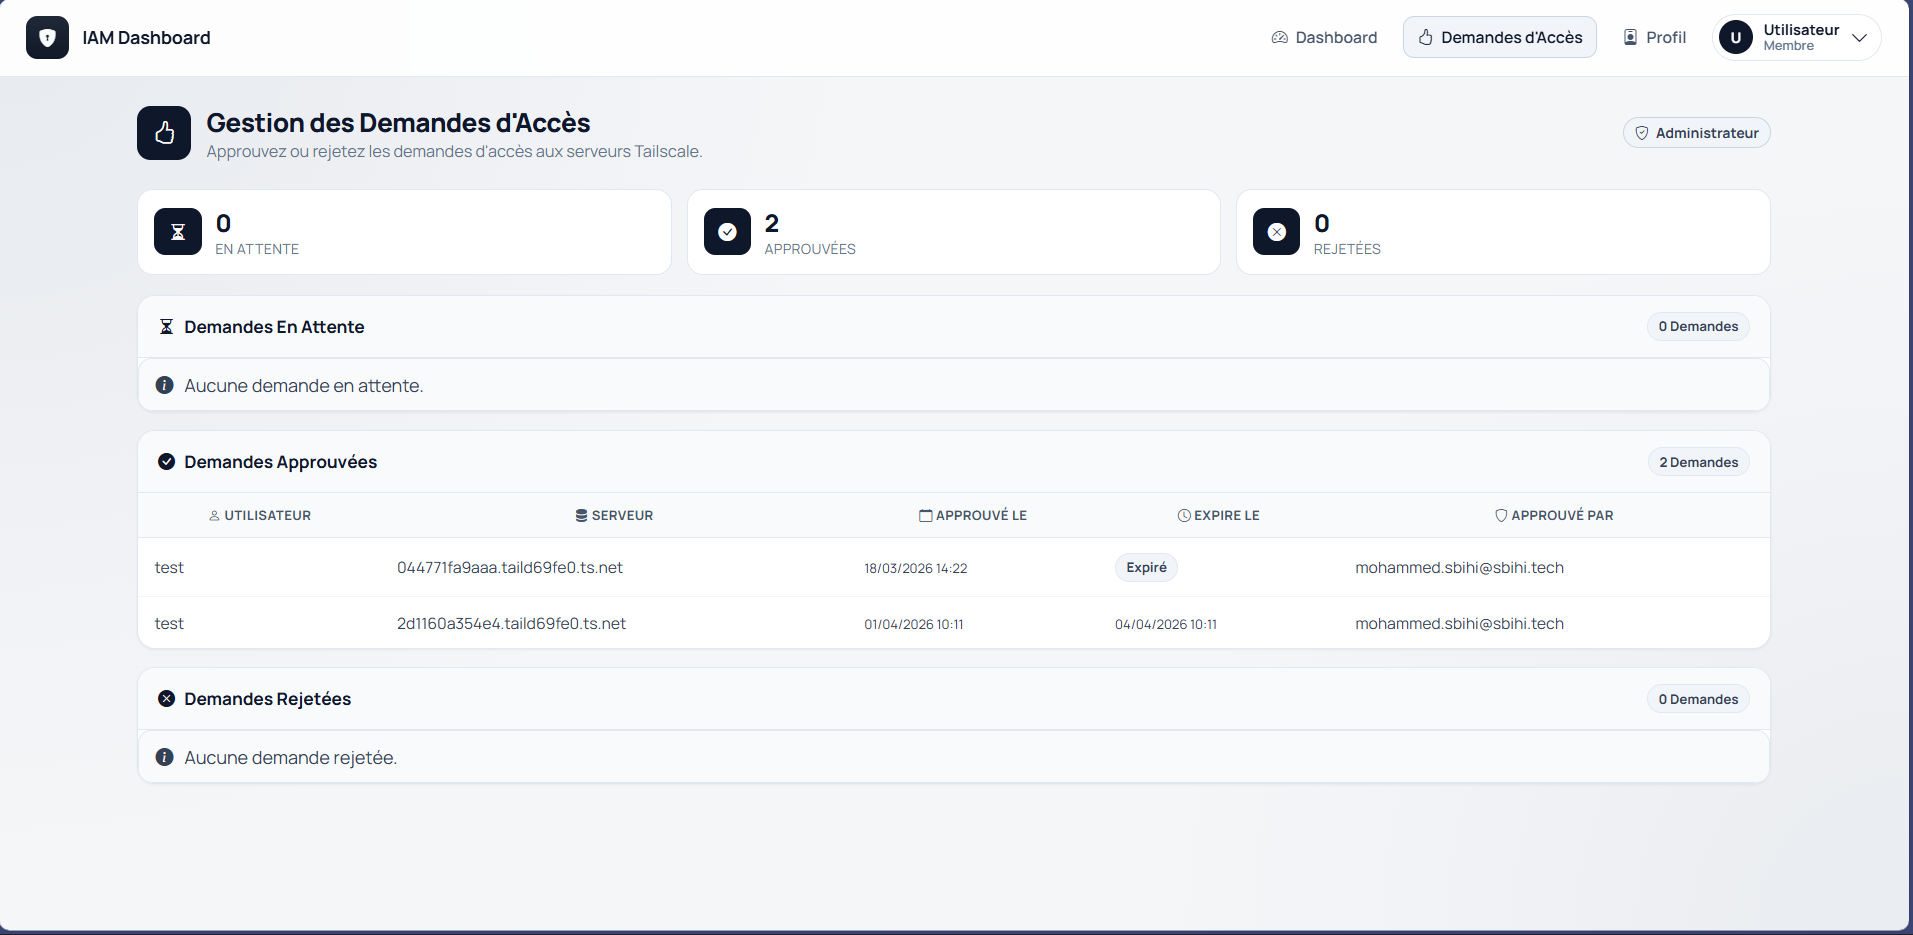
\includegraphics[width=0.95\textwidth]{images/apres_approbation_by_admin_from_admin_side.png}
	\caption{Etat de la demande apres approbation vu depuis l'interface administrateur.}
	\label{fig:admin-after-approval}
\end{figure}
L'etat post-approbation confirme la coherence entre action admin et resultat systeme. La demande est historisee avec son nouveau statut, ce qui simplifie les verifications ulterieures en audit interne.

\begin{figure}[H]
	\centering
	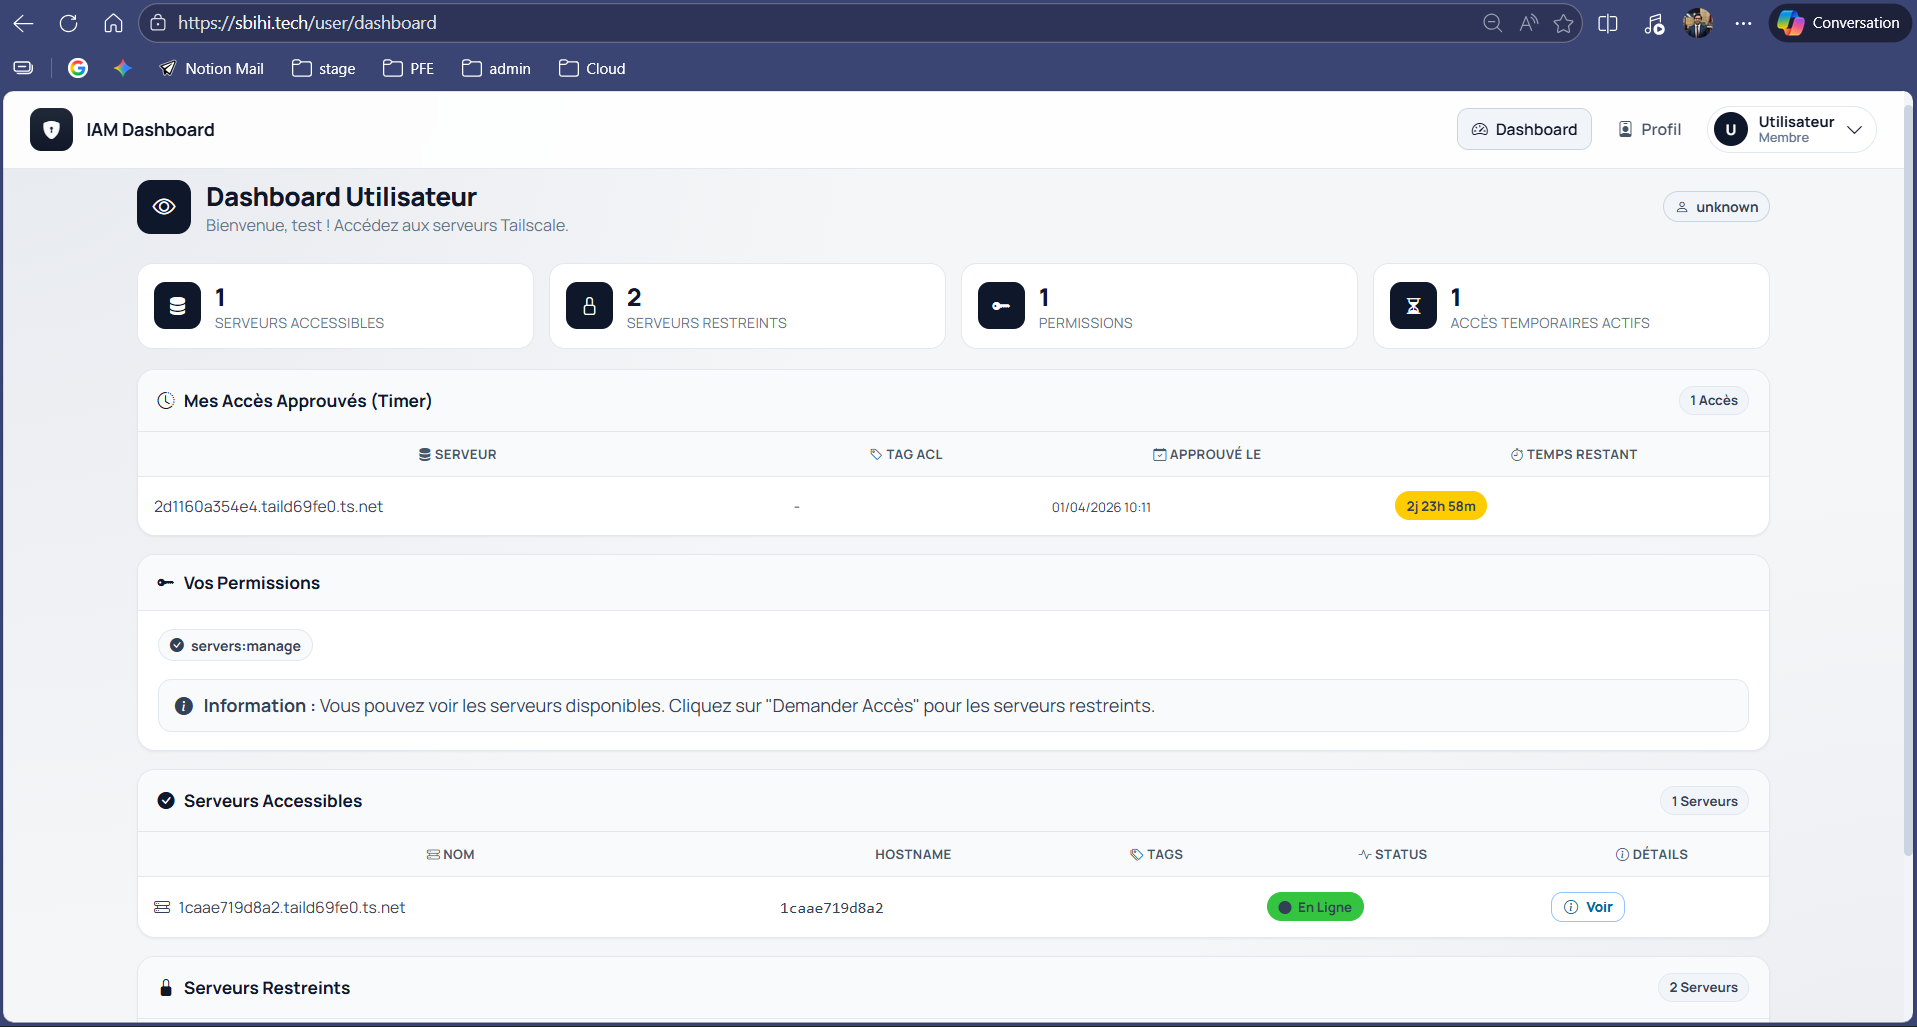
\includegraphics[width=0.95\textwidth]{images/acces_approuver_coter_user.png}
	\caption{Etat cote utilisateur apres validation admin: acces marque comme approuve avec fenetre temporelle active.}
	\label{fig:user-after-approval}
\end{figure}
Le retour cote utilisateur est un element important de gouvernance: il confirme l'etat de la demande et rend visible la temporalite de l'acces, ce qui reduit les ambiguïtés operationnelles.

\section{Moteur JIT Python (ACL\_work)}
Le moteur JIT est implemente dans les scripts Python du dossier \texttt{ACL\_work}.

Fonctions principales:
\begin{itemize}
	\item \texttt{approve\_access\_request(...)}: activation de la regle ACL et mise a jour de la base;
	\item \texttt{revoke\_access\_request(...)}: suppression de la regle ACL et mise a jour de statut;
	\item \texttt{cleanup\_expired\_requests(...)}: nettoyage periodique des droits expires.
\end{itemize}

Le script de maintenance periodique (cron) garantit qu'aucun acces privilegie ne reste actif au-dela de sa duree autorisee.

\begin{figure}[H]
	\centering
	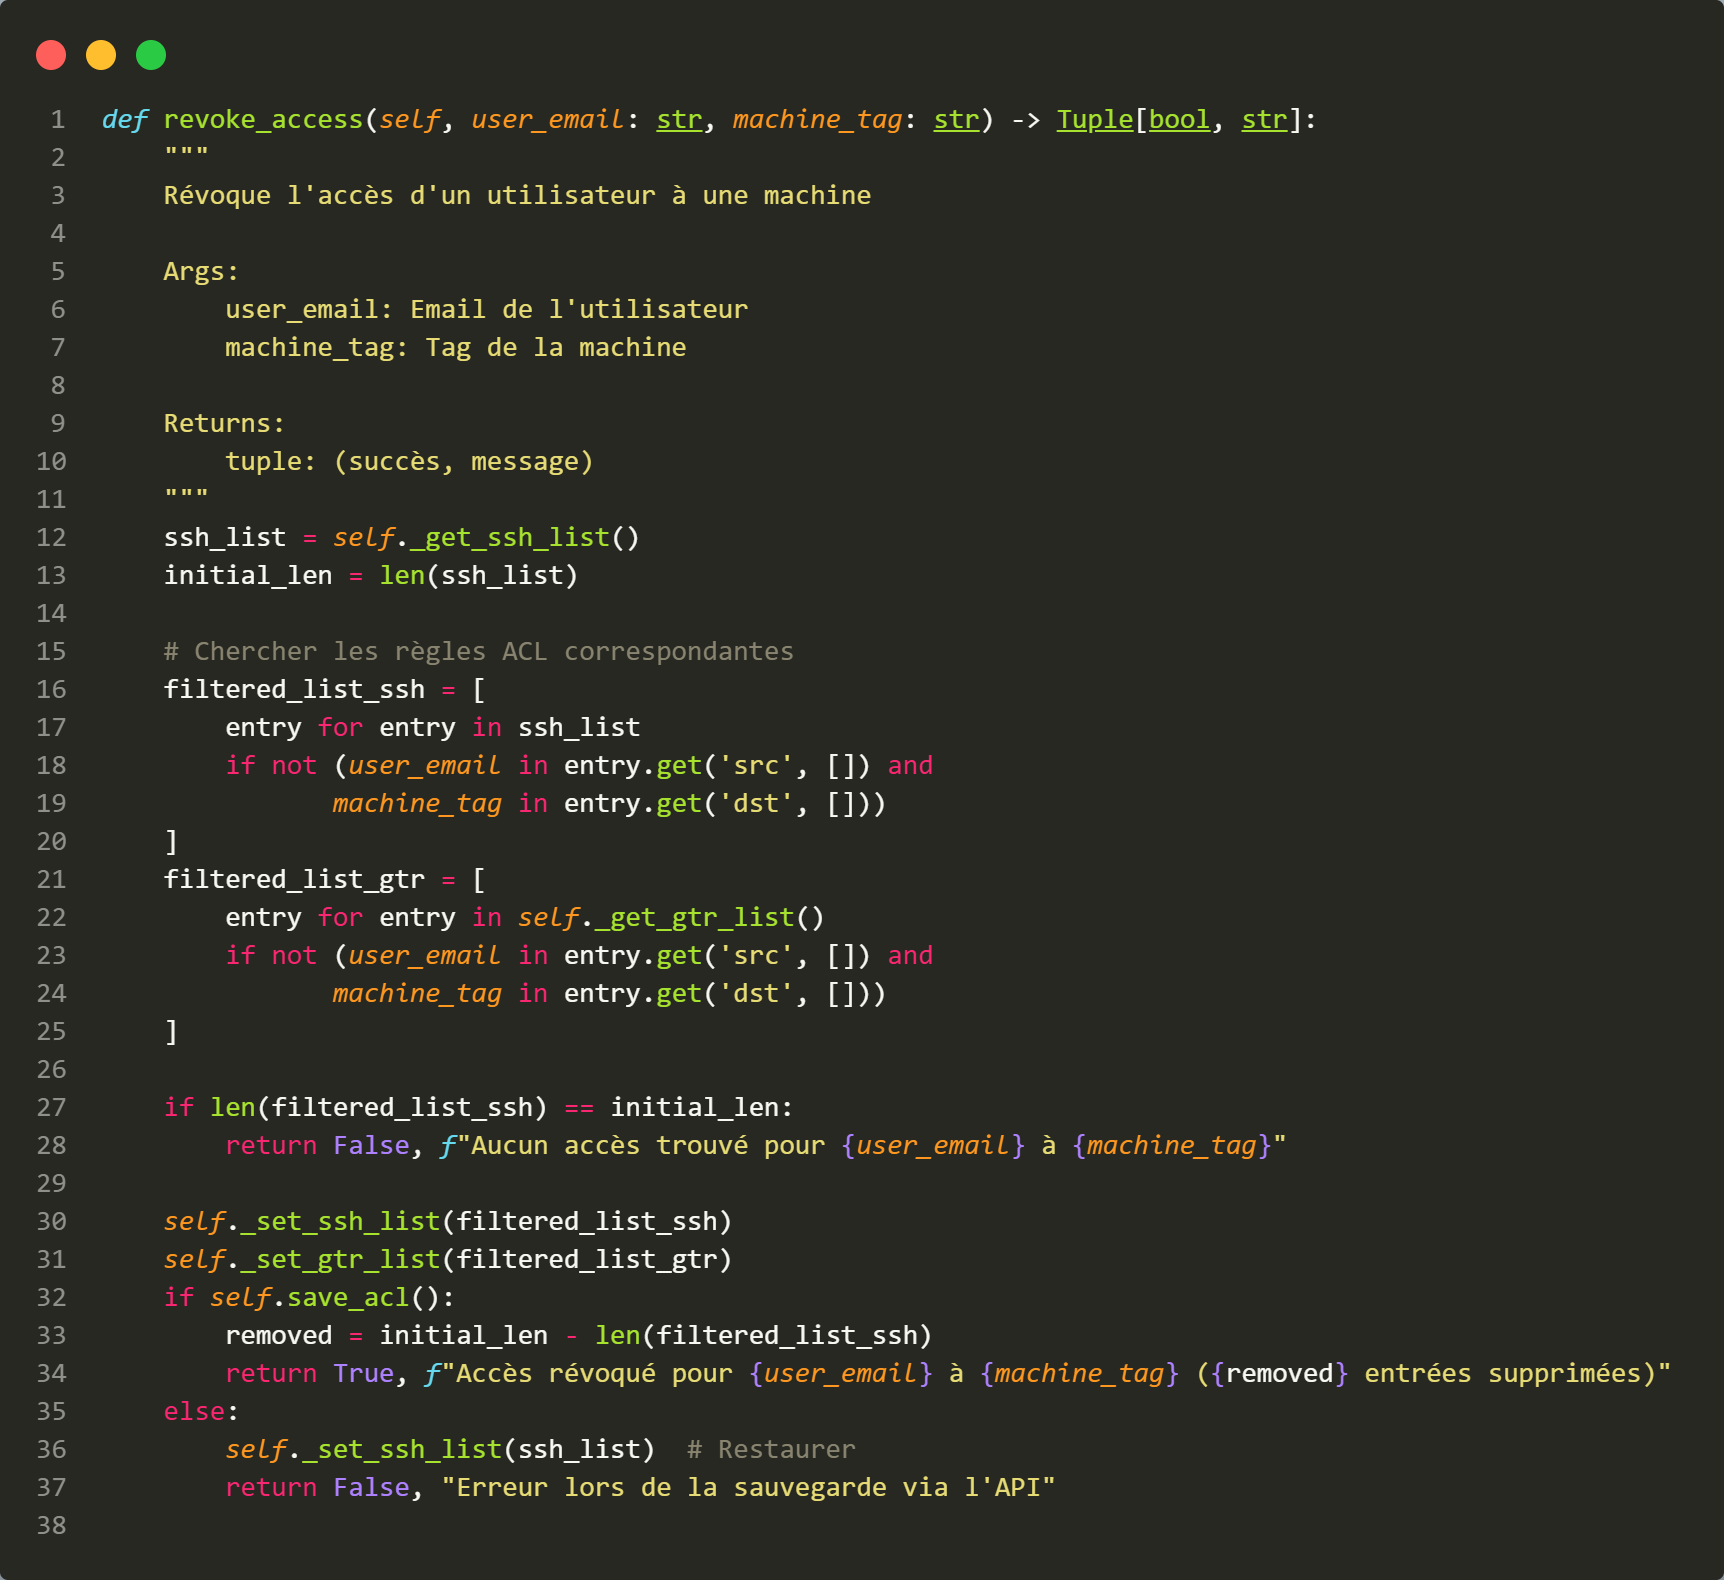
\includegraphics[width=0.95\textwidth]{images/revove_acces_fonction.png}
	\caption{Fonction de revocation d'acces dans le moteur Python: suppression des regles ACL SSH/Grant et gestion du rollback en cas d'echec API.}
	\label{fig:python-revoke-function}
\end{figure}
Le code de revocation montre une logique defensive: suppression ciblee des regles, tentative de sauvegarde via API, puis restauration en cas d'echec. Ce mecanisme limite le risque d'etat incoherent entre base applicative et politique ACL reelle.

\section{Wazuh et observabilite}
Wazuh apporte la visibilite necessaire pour l'audit et la detection d'anomalies.

Les informations attendues dans cette couche sont:
\begin{itemize}
	\item evenements d'authentification et d'echec MFA;
	\item traces d'actions admin (approbation, refus, revocation);
	\item journaux d'acces et d'expiration utiles a la conformite.
\end{itemize}

\subsection{Logging sur les machines cibles}
Sur la machine cible SSH conteneurisee, le journal applicatif de session est force dans \texttt{/var/log/auth.log}. Le script d'entree active \texttt{rsyslog}, cree le fichier de log et injecte un \texttt{PROMPT\_COMMAND} Bash qui journalise chaque commande executee, avec l'identite Tailscale resolue dynamiquement.

\begin{figure}[H]
	\centering
	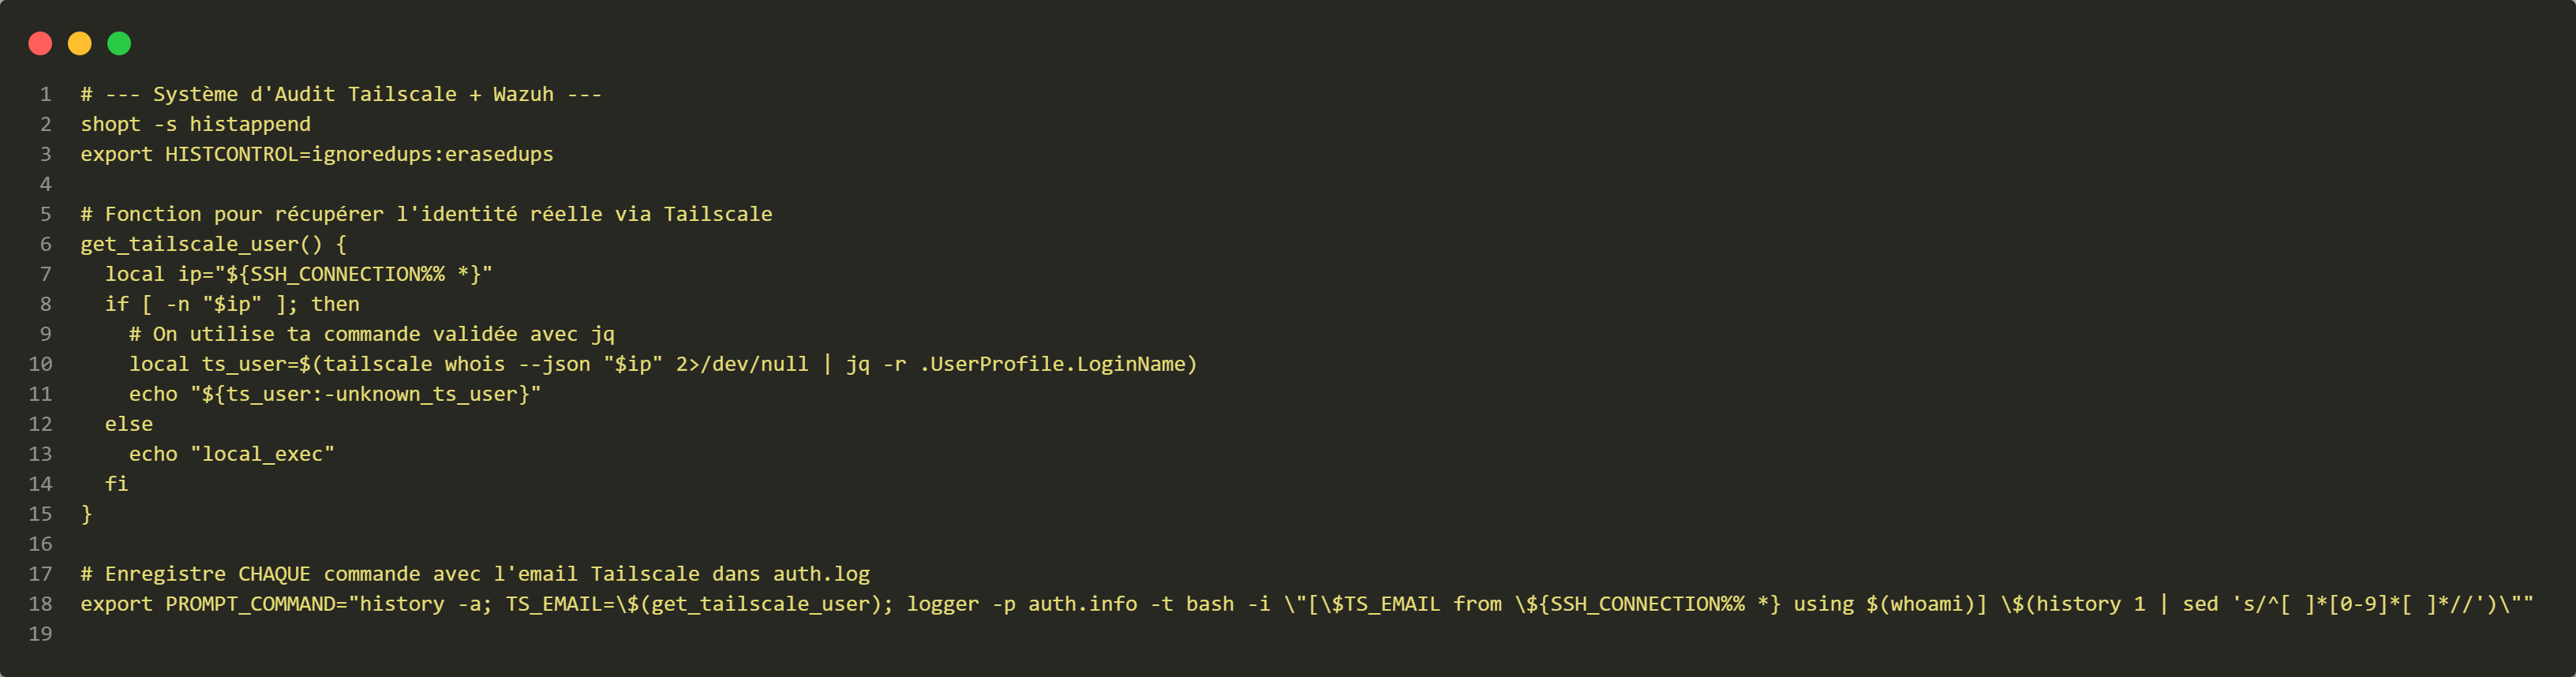
\includegraphics[width=0.96\textwidth]{images/sys_audit.png}
	\caption{Code de journalisation SSH.}
	\label{fig:wazuh-ssh-command-audit}
\end{figure}

Cette approche garantit que les commandes shell sensibles ne restent pas uniquement dans l'historique local utilisateur: elles sont centralisees dans un journal systeme exploitable par l'agent Wazuh.

\subsection{Configuration Wazuh agent et manager}
Le manager Wazuh distribue une configuration agent partagee afin de collecter explicitement \texttt{/var/log/auth.log} avec le format \texttt{syslog}.

\begin{lstlisting}[language=XML, basicstyle=\ttfamily\small]
<agent_config>
  <localfile>
    <log_format>syslog</log_format>
    <location>/var/log/auth.log</location>
  </localfile>
</agent_config>
\end{lstlisting}

Le deploiement Docker du manager monte en plus les decoders, les regles personnalisees et \texttt{agent.conf}, ce qui permet une chaine complete ingestion -> parsing -> alerting sans reconstruire l'image officielle.

\begin{lstlisting}[language=bash, basicstyle=\ttfamily\small]
./decoders/bash_decoder.xml:/var/ossec/etc/decoders/bash_decoder.xml
./rules/bash_rules.xml:/var/ossec/etc/rules/bash_rules.xml
./agents/agent.conf:/var/ossec/etc/shared/default/agent.conf
\end{lstlisting}

\subsection{Decodage et regles d'alerte Bash}
Le decoder \texttt{bash\_audit} extrait les champs utiles (utilisateur Tailscale, source, commande), puis les regles elevent la severite pour les commandes d'administration telles que \texttt{apt}, \texttt{dpkg}, \texttt{rm}, \texttt{nano} et \texttt{vi}.

Ce mecanisme relie directement l'activite shell de la machine cible au SIEM, avec un contexte identite + commande exploitable pour l'audit et la reponse a incident.

\begin{figure}[H]
	\centering
	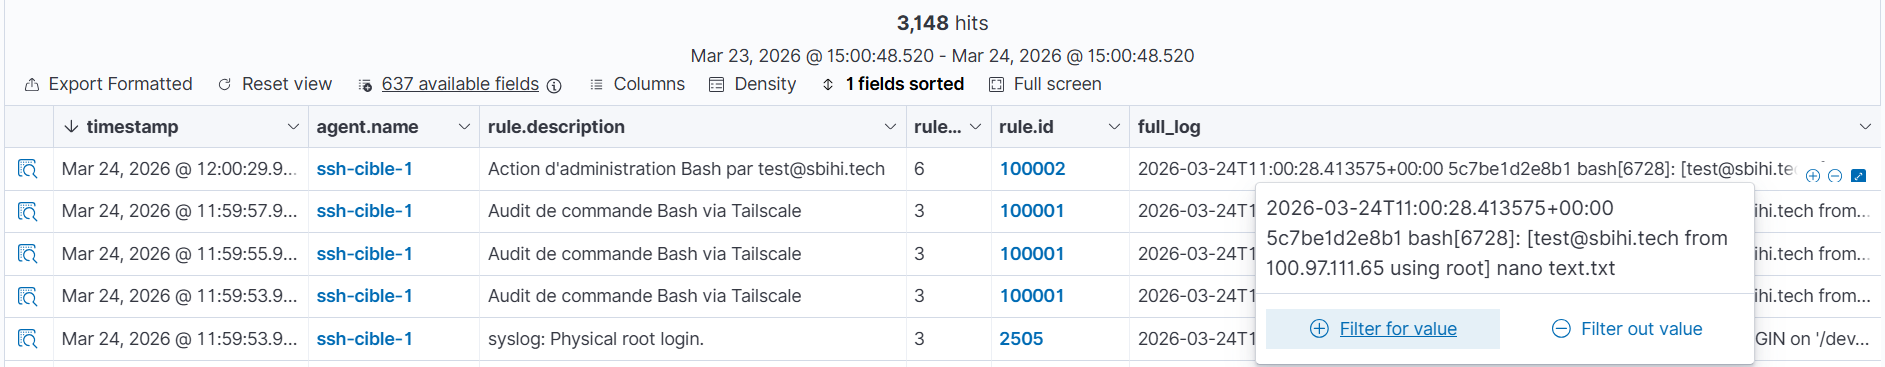
\includegraphics[width=0.96\textwidth]{images/wazuh_log_from ssh showing what the user did in after login to the ssh cible .png}
	\caption{Preuve de centralisation Wazuh: traces de commandes SSH executees sur la machine cible avec contexte utilisateur.}
	\label{fig:wazuh-ssh-command-audit}
\end{figure}
La capture montre la finalite du pipeline: ce qui est tape sur la machine cible est visible dans Wazuh, avec un niveau de detail suffisant pour la tracabilite de conformite et l'investigation technique.

\section{Conclusion du chapitre}
L'implementation par composant confirme la faisabilite technique de la chaine Zero Trust: identite forte, activation conditionnelle des droits, limitation temporelle et tracabilite. Le chapitre suivant valide ces mecanismes par des scenarios de test structures.
